\chapter{Experimental Results from Corroded Rebar Specimens}
\label{chap-four}
Presented in this chapter are the findings of the experimental program just described. The two types of tests are addressed independently. The chapter opens with a presentation of the obtained corrosion levels for the reinforcing steel specimens using two different approaches: 1) using the mass loss method and 2) using the geometrical reduction of the effective diameter of the reinforcing steel via 3D scanning. 

The chapter continues with the presentation of the tensile test results obtained from reinforcing steel at corrosion levels ranging from 0\% - 20\%. Following the relationships between the yield strength, ultimate strength, and uniform axial elongation, the corrosion levels are studied. The results from the tension tests are coherent with previous research, in which as the corrosion level increases, the effective mechanical properties of the material change. 

Similarly, for the buckled bar tension (BBT) tests, the results for corrosion levels ranging from 0\% - 20\% are presented. To the author’s knowledge, this is the first of this type of test performed on corroded reinforcing steel. The results show that there is a decrease in the maximum bending strain as the corrosion level increases. These results will explain the observed reduction in displacement capacity of corroded reinforced concrete members. 

In addition, to tension tests and BBT tests, the experimental program was interested in observing if there were any changes at the microstructural level and if a concentrated chloride attack induced the failure in any way. Therefore, observations and data that were obtained from a scanning electron microscope (SEM) will be shown.

Finally, results from the tension and BBT tests on corroded rebar with removed surface imperfections are shown. The results show that the virgin material properties remained unchanged, and the results observed on corroded rebars are due to the geometrical imperfections induced by the corrosion.

\section{Measurement of Corrosion Level}

\subsection{Mass loss method}

The corrosion level of each specimen was measured after the time to corrode them had passed. The procedure consisted in removing the corrosion products from the surface of the specimens. The bars were then weighted and the mass loss was measured. Finally, the corrosion level is defined as the mass loss divided by the initial mass, as shown in \eref{eq:mass_loss_CL}.

\begin{equation}
    CL=\frac{m_{initial}-m_{final}}{m_{initial}}
    \label{eq:mass_loss_CL}
\end{equation}

Table \ref{tab:CL_mass_loss_method} shows the resulting corrosion level using \eref{eq:mass_loss_CL}. The resulting corrosion was significantly close to the target corrosion levels, and proved that the test setup successfully achieved the intended corrosion levels. In addition, one parent specimen (containing three specimen subsets) for CL=15\% did not achieve the intended corrosion level, mainly due to a faulty welding of the stainless steel wire to the rebar. These bars were repurposed for tension tests of turned down rebars.

\begin{table}[]
\caption{Corroded Level measured from mass loss in gauge length}
\label{tab:CL_mass_loss_method}
\begin{center}
\begin{tabular}{lcccc}
Specimen ID & Initial mass (g) & Final mass (g) & Mass loss (g) & CL (\%) \\ \hline
CL5-T-1\_3    & 1260.8           & 1197.5         & 63.3          & 5.0\%   \\
CL5-BBT-1\_3  & 1249.6           & 1199.8         & 49.9          & 4.0\%   \\
CL5-BBT-4-6   & 1255.3           & 1192.9         & 62.4          & 4.9\%   \\
CL10-T-1\_3   & 1244.0           & 1122.6         & 121.3         & 9.8\%   \\
CL10-BBT-1\_3 & 1248.7           & 1131.7         & 117.0         & 9.4\%   \\
CL10-BBT-4-6  & 1258.7           & 1143.1         & 115.7         & 9.2\%   \\
CL15-BBT-1\_3 & 1217.9           & 1052.3         & 165.6         & 13.6\%  \\
CL15-BBT-4-6  & 1265.5           & 1095.4         & 170.1         & 13.4\%  \\
CL20-T-1\_3   & 1251.2           & 1022.9         & 228.4         & 18.3\%  \\
CL20-BBT-1\_3 & 1245.1           & 1018.3         & 226.8         & 18.2\%  \\
CL20-BBT-4\_6  & 1272.3           & 1013.8         & 258.5         & 20.3\% 
\end{tabular}
\end{center}
\end{table}

\subsection{3D Scanning Method}

The 3d scan Faro Arm was used to obtain 3D models of the corroded rebars to determine the effective diameter in the gauge length of the specimens. The effective diameter was used to determine the stress strain relationships and the bending strain in the rebars. \fref{fig:3D_scans_sample} shows a sample of the 3D scans for CL=15\% and CL=20\%. This figure shows that the 3D scans captured the imperfections on the surface of the rebars with a high level of precision. 

\begin{figure}[htbp]
	\centering
	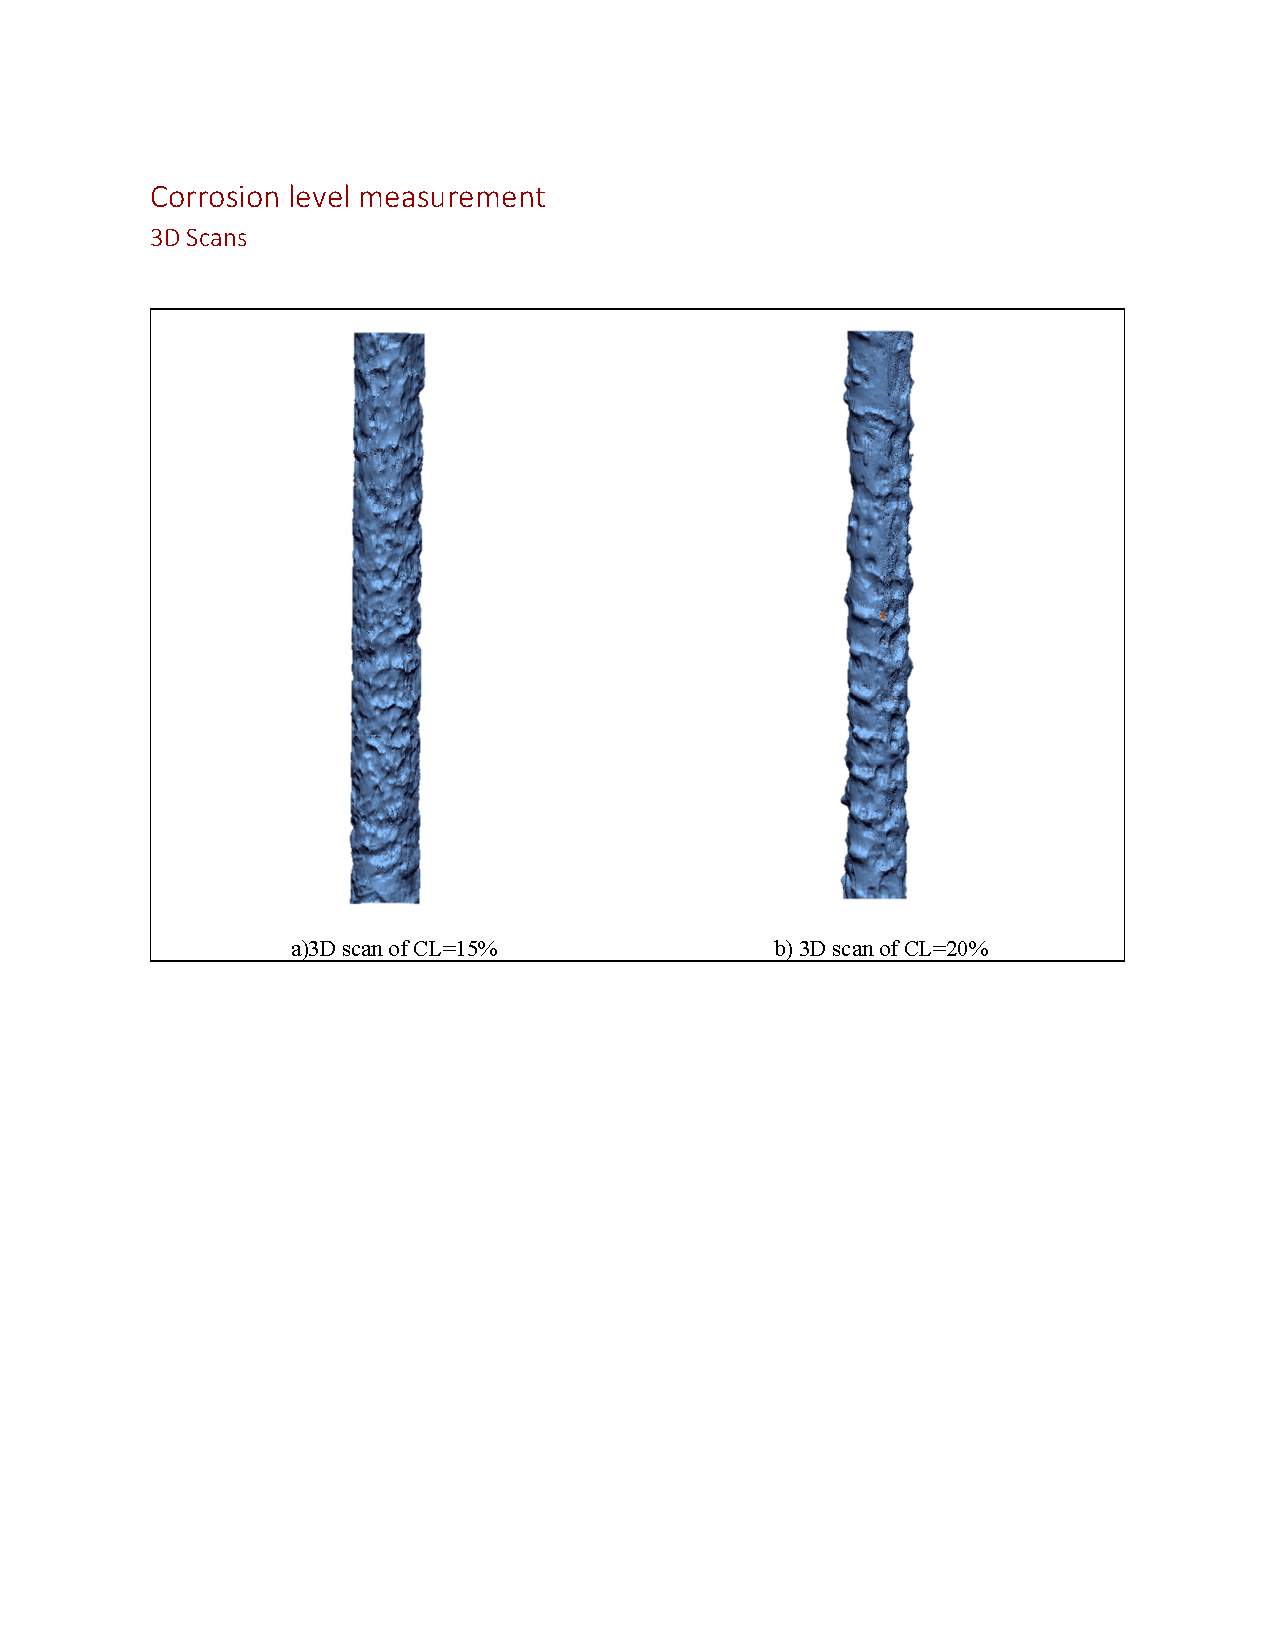
\includegraphics[width=0.6\textwidth]{VAC Thesis 2.0/Chapter-4/figs/3dScans_sample.pdf}
	\caption{Sample of 3D scans obtained for CL=15\% and CL=20\%}
    \label{fig:3D_scans_sample}
\end{figure}

From the 3D model, the volume ($V$) in the gauge length was obtained, and assuming a cylindrical volume, the effective diameter ($d_{eff}$) can be obtained as expressed in \eref{eq:eff_diameter}, where $L_{o}$ is the length of the scanned gauge length. With the effective diameter, the corrosion level can be estimated as shown in \eref{eq:CL_diameter}, where $d_{o}$ refers to the initial diameter. In the case of the specimens of this study, it corresponds to  $d_{o}=19mm (0.75 in)$

\begin{equation}
    d_{eff}=\frac{V}{\frac{1}{4}\pi L_{o}}
    \label{eq:eff_diameter}
\end{equation}

\begin{equation}
    CL=1-(\frac{d_{eff}}{d_{o}})^2
    \label{eq:CL_diameter}
\end{equation}

The data collected from the 3D scans is summarized in \ref{tab:CL_3D_scans}. The results shown below demonstrate that the corrosion level (CL) measured using this approach matches well with the intended corrosion level.

\begin{table}[htpb]
\caption{Corrosion levels (CL) measured from 3D scans in gauge length}
\label{tab:CL_3D_scans}
\begin{tabularx}{1.0\textwidth} { 
   >{\raggedright\arraybackslash}X 
   >{\centering\arraybackslash}X 
  >{\centering\arraybackslash}X >{\centering\arraybackslash}X >{\centering\arraybackslash}X >{\centering\arraybackslash}X}
Specimen ID    & Volume ($mm^{3}$) & Height \newline ($mm$) & Diameter ($mm$) & 3D Scans CL (\%) & Average CL (\%) \\ \hline
CL5-T-1    & 47702                          & 179         & 18.4          & 6.50\%                        & \multirow{3}{*}{6.00\%}  \\
CL5-T-2    & 47388                          & 176.5       & 18.5          & 5.80\%                        &                          \\
CL5-T-3    & 44696                          & 166.1       & 18.5          & 5.60\%                        &                          \\
CL5-BBT-1  & 48389                          & 178.2       & 18.6          & 4.70\%                        & \multirow{3}{*}{4.80\%}  \\
CL5-BBT-2  & 48903                          & 178.2       & 18.7          & 3.70\%                        &                          \\
CL5-BBT-3  & 47876                          & 178.6       & 18.5          & 5.90\%                        &                          \\
CL5-BBT-4  & 48618                          & 178         & 18.6          & 4.20\%                        & \multirow{3}{*}{4.70\%}  \\
CL5-BBT-5  & 47984                          & 178.3       & 18.5          & 5.60\%                        &                          \\
CL5-BBT-6  & 48750                          & 178.6       & 18.6          & 4.20\%                        &                          \\
CL10-T-1   & 45281                          & 178.8       & 18.0          & 11.10\%                       & \multirow{3}{*}{11.30\%} \\
CL10-T-2   & 44658                          & 178.1       & 17.9          & 12.00\%                       &                          \\
CL10-T-3   & 45359                          & 178.1       & 18.0          & 10.60\%                       &                          \\
CL10-BBT-1 & 45815                          & 178.5       & 18.1          & 9.90\%                        & \multirow{3}{*}{9.70\%}  \\
CL10-BBT-2 & 47595                          & 182         & 18.2          & 8.20\%                        &                          \\
CL10-BBT-3 & 45364                          & 178.8       & 18.0          & 11.00\%                       &                          \\
CL10-BBT-4 & 46486                          & 178.9       & 18.2          & 8.80\%                        & \multirow{3}{*}{10.00\%} \\
CL10-BBT-5 & 45676                          & 178.7       & 18.0          & 10.30\%                       &                          \\
CL10-BBT-6 & 45353                          & 178.2       & 18.0          & 10.70\%                       &                          \\
CL15-BBT-1 & 43119                          & 178.8       & 17.5          & 15.40\%                       & \multirow{3}{*}{15.30\%} \\
CL15-BBT-2 & 41474                          & 169.7       & 17.6          & 14.20\%                       &                          \\
CL15-BBT-3 & 35373                          & 148.1       & 17.4          & 16.20\%                       &                          \\
CL15-BBT-4 & 40485                          & 168.1       & 17.5          & 15.50\%                       & \multirow{3}{*}{15.00\%} \\
CL15-BBT-5 & 38297                          & 160.4       & 17.4          & 16.20\%                       &                          \\
CL15-BBT-6 & 41103                          & 166.4       & 17.7          & 13.30\%                       &                          \\
CL20-T-1   & 40786                          & 178.2       & 17.1          & 19.70\%                       & \multirow{3}{*}{20.30\%} \\
CL20-T-2   & 36577                          & 163.4       & 16.9          & 21.40\%                       &                          \\
CL20-T-3   & 40864                          & 178.6       & 17.1          & 19.70\%                       &                          \\
CL20-BBT-1 & 41038                          & 178.9       & 17.1          & 19.50\%                       & \multirow{3}{*}{19.50\%} \\
CL20-BBT-2 & 37452                          & 164.3       & 17.0          & 20.00\%                       &                          \\
CL20-BBT-3 & 41186                          & 178.5       & 17.1          & 19.00\%                       &                          \\
CL20-BBT-4 & 39645                          & 178.4       & 16.8          & 22.00\%                       & \multirow{3}{*}{21.80\%} \\
CL20-BBT-5 & 35364                          & 158.4       & 16.9          & 21.70\%                       &                          \\
CL20-BBT-6 & 39786                          & 178.1       & 16.9          & 21.60\%                       &                                                                             
\end{tabularx}
\end{table}

\subsection{Comparison of Corrosion Level (CL) Measurements Mass Loss vs 3D Scanning Methods}

Finally, the results from obtaining the corrosion level using the mass loss approach and the 3D scans are compared in \fref{fig:3dscans_vs_massloss}.4.2. The results from both approaches match very well, and the discrepancy from both could be due to more localized corrosion measured in the single specimens as opposed to those measured in the parent bar specimen, as was the case for the mass loss methodology. These results provided us with the opportunity to use the measured effective diameter from the 3D scans in the tension tests and BBT tests described in the following sections.

\begin{figure}[htbp]
	\centering
    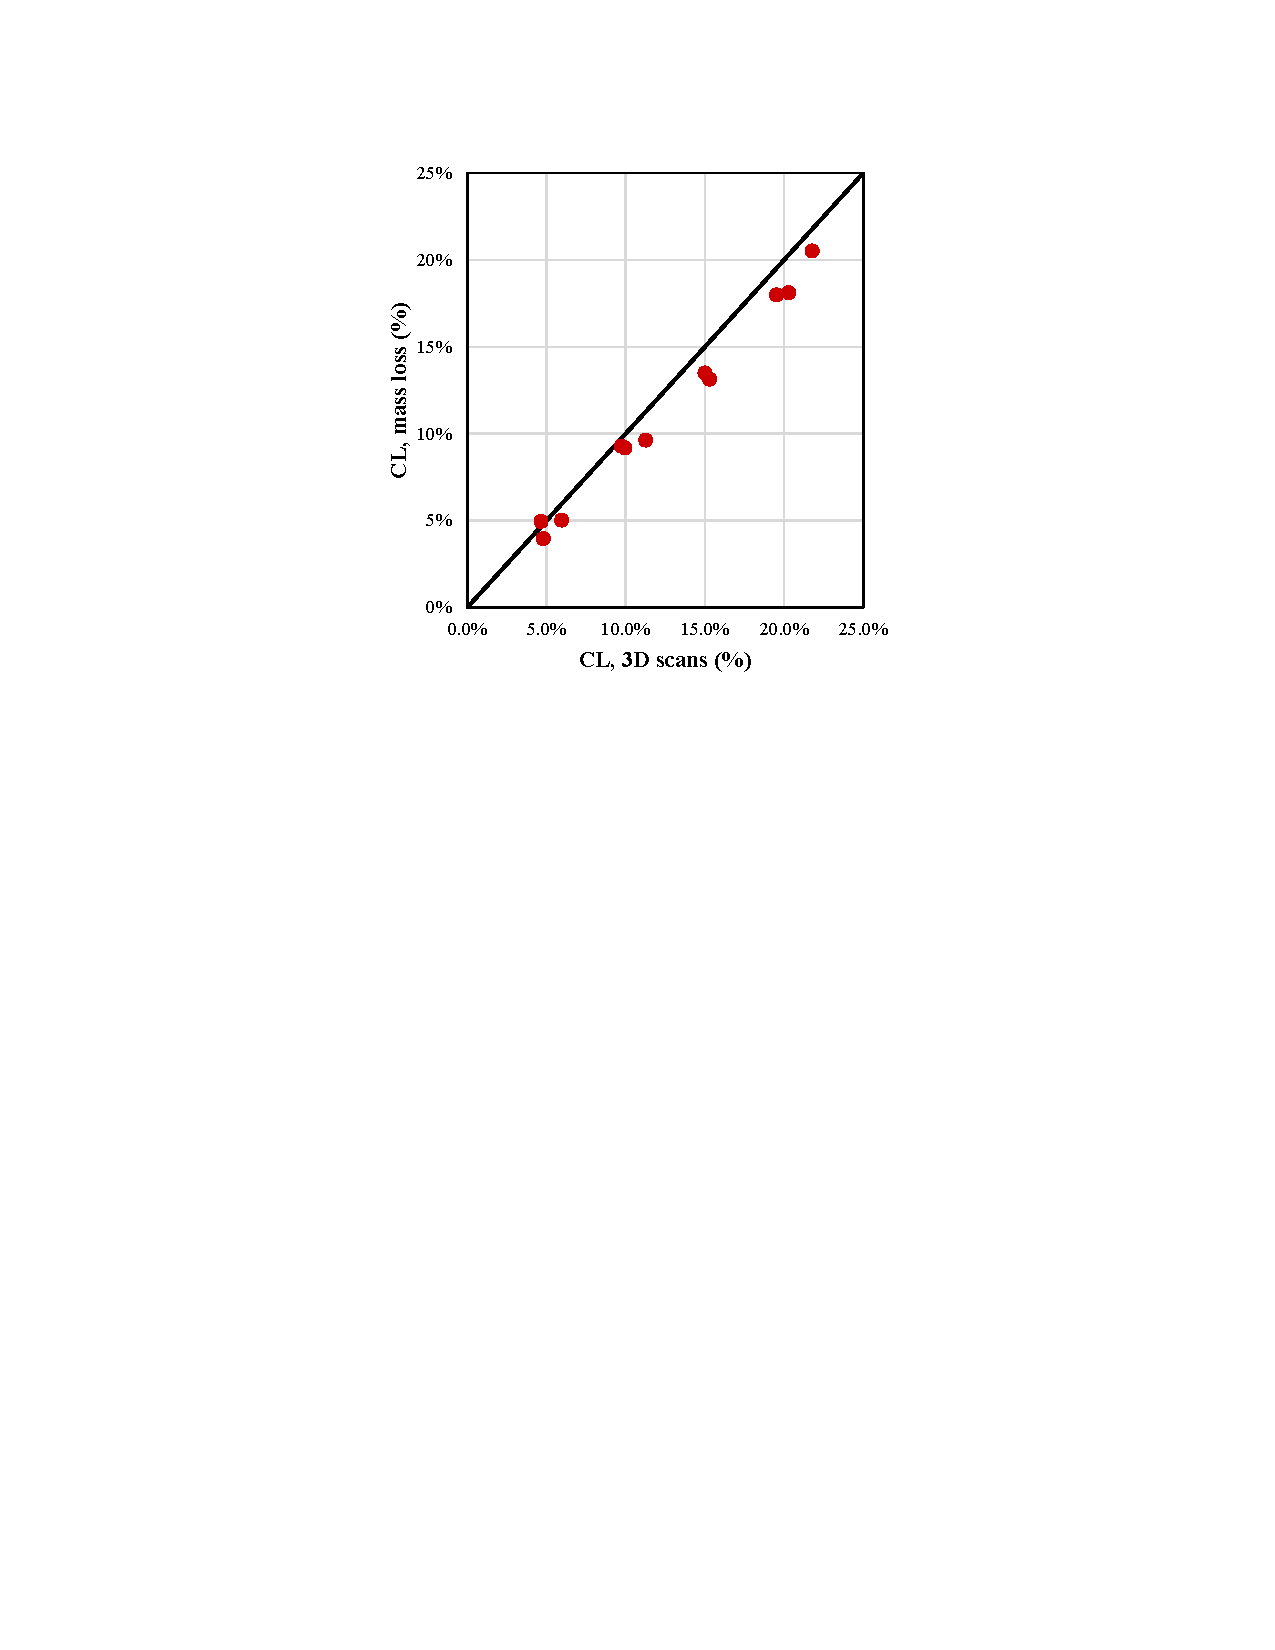
\includegraphics[width=0.5\textwidth]{VAC Thesis 2.0/Chapter-4/figs/3dscans_vs_massloss.pdf}
	\caption{Corrosion level (CL) measured using mass loss method vs 3D scans}
\label{fig:3dscans_vs_massloss}
\end{figure}

\newpage
\section{Tension Tests}

As described in Chapter \ref{chap-three}, the bars were loaded in tension using the universal testing machine (UTM). The data collected corresponded to the Force using the UTM, and the Optotrack system was used to calculate the strain.

While no differences in the test procedure for corroded and uncorroded tests were made, it was observed that during the tests, the fracture usually occurred close to the grips, as shown in \fref{fig:TensionTest_NoNecking} 
b). It is hypothesized that this is due to the sudden change in the cross section and the imperfections on the rebars. The strains used in this study correspond to the strain gauges located adjacent to the fracture. The fracture of these tests were brittle in nature, since the appearance of necking was not significantly observable, as shown in  \fref{fig:TensionTest_NoNecking} c).

\begin{figure}[htbp]
	\centering
	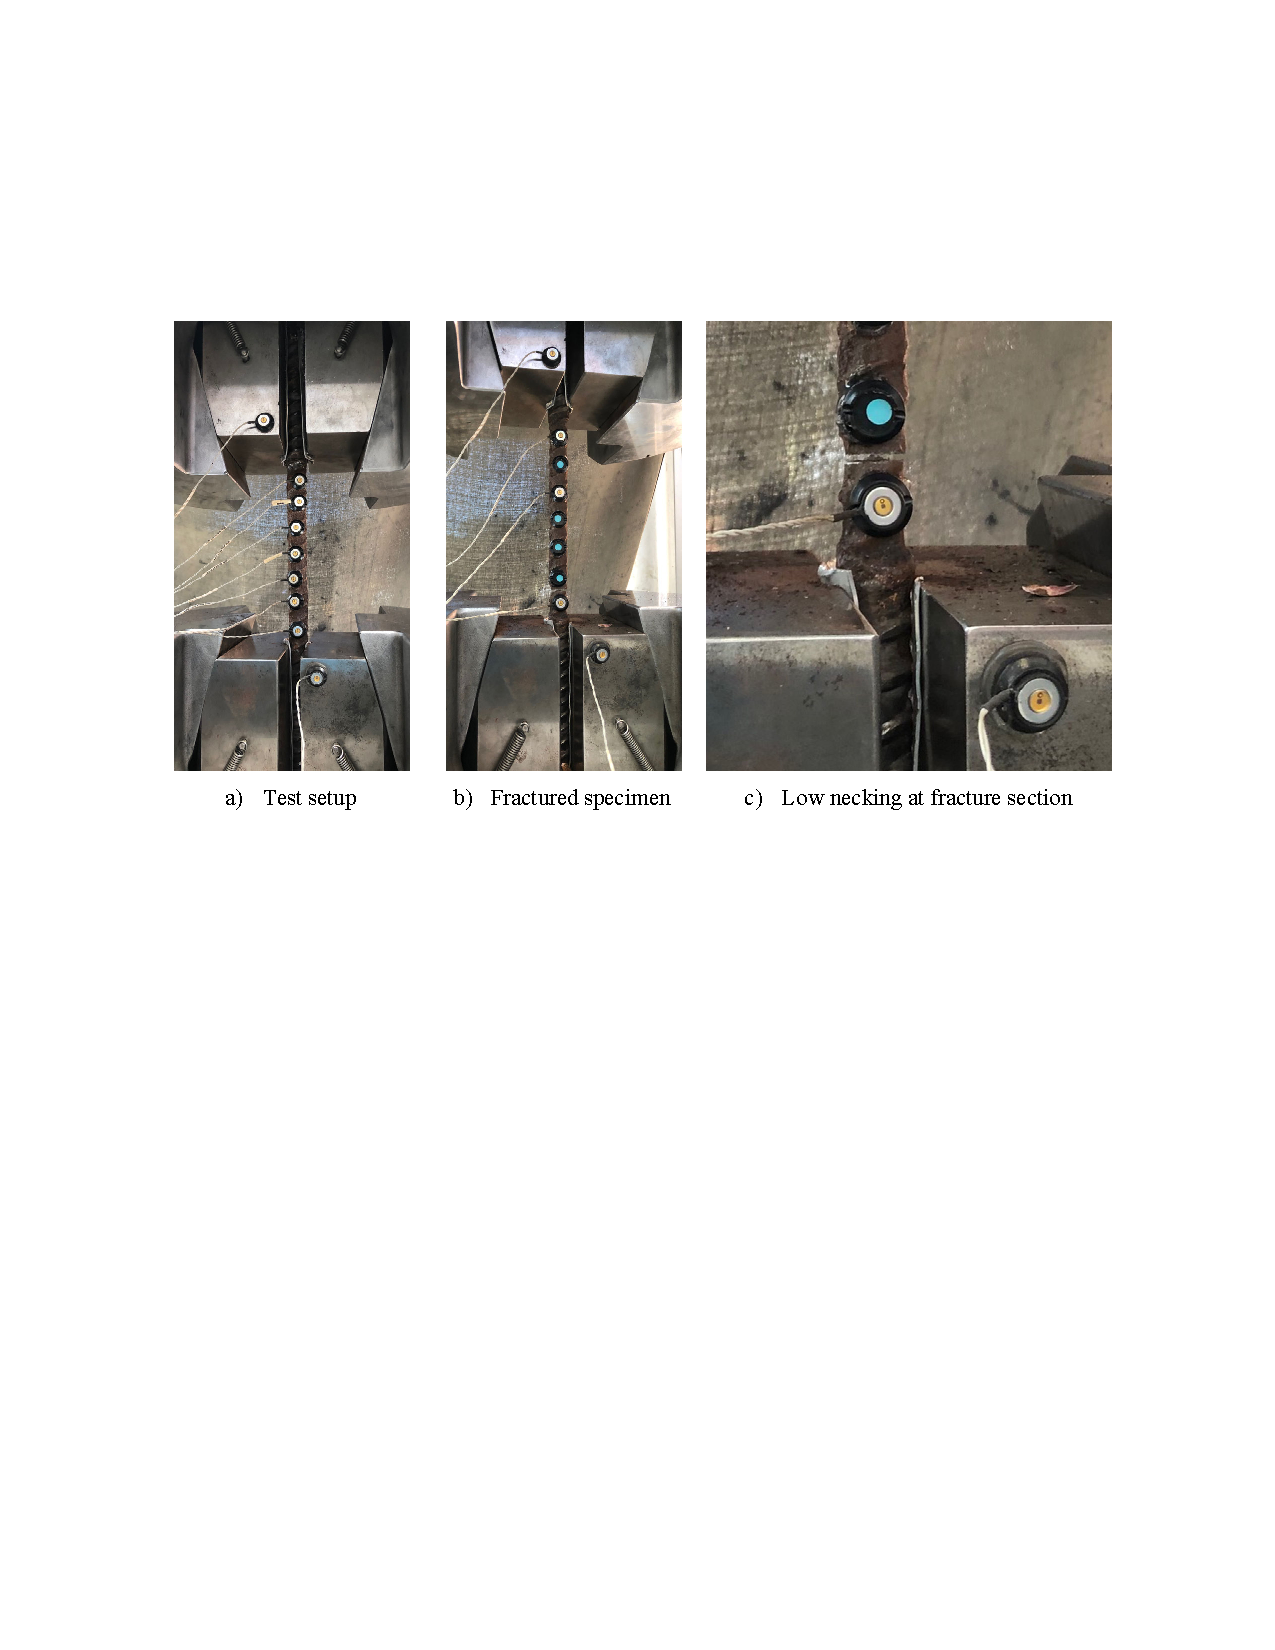
\includegraphics[width=0.7\textwidth]{VAC Thesis 2.0/Chapter-4/figs/TensionTest_images.pdf}
	\caption{Tension test setup and fracture observations}
	\label{fig:TensionTest_NoNecking}
\end{figure}

A summary of the stress strain behavior for the corroded rebars is shown in \fref{fig:TensionTestResults_StressStrain}. . In addition, the results obtained for pristine bars from research performed by Barcley et al.  \cite{Barcley2018}, and Overby et al. \cite{Overby2016}. In general, from \fref{fig:TensionTestResults_StressStrain} it can be observed that as corrosion increases, the effective yield strength, ultimate strength, and uniform elongation tend to decrease. These variables are explained in more detail below.

\begin{figure}[htbp]
	\centering
	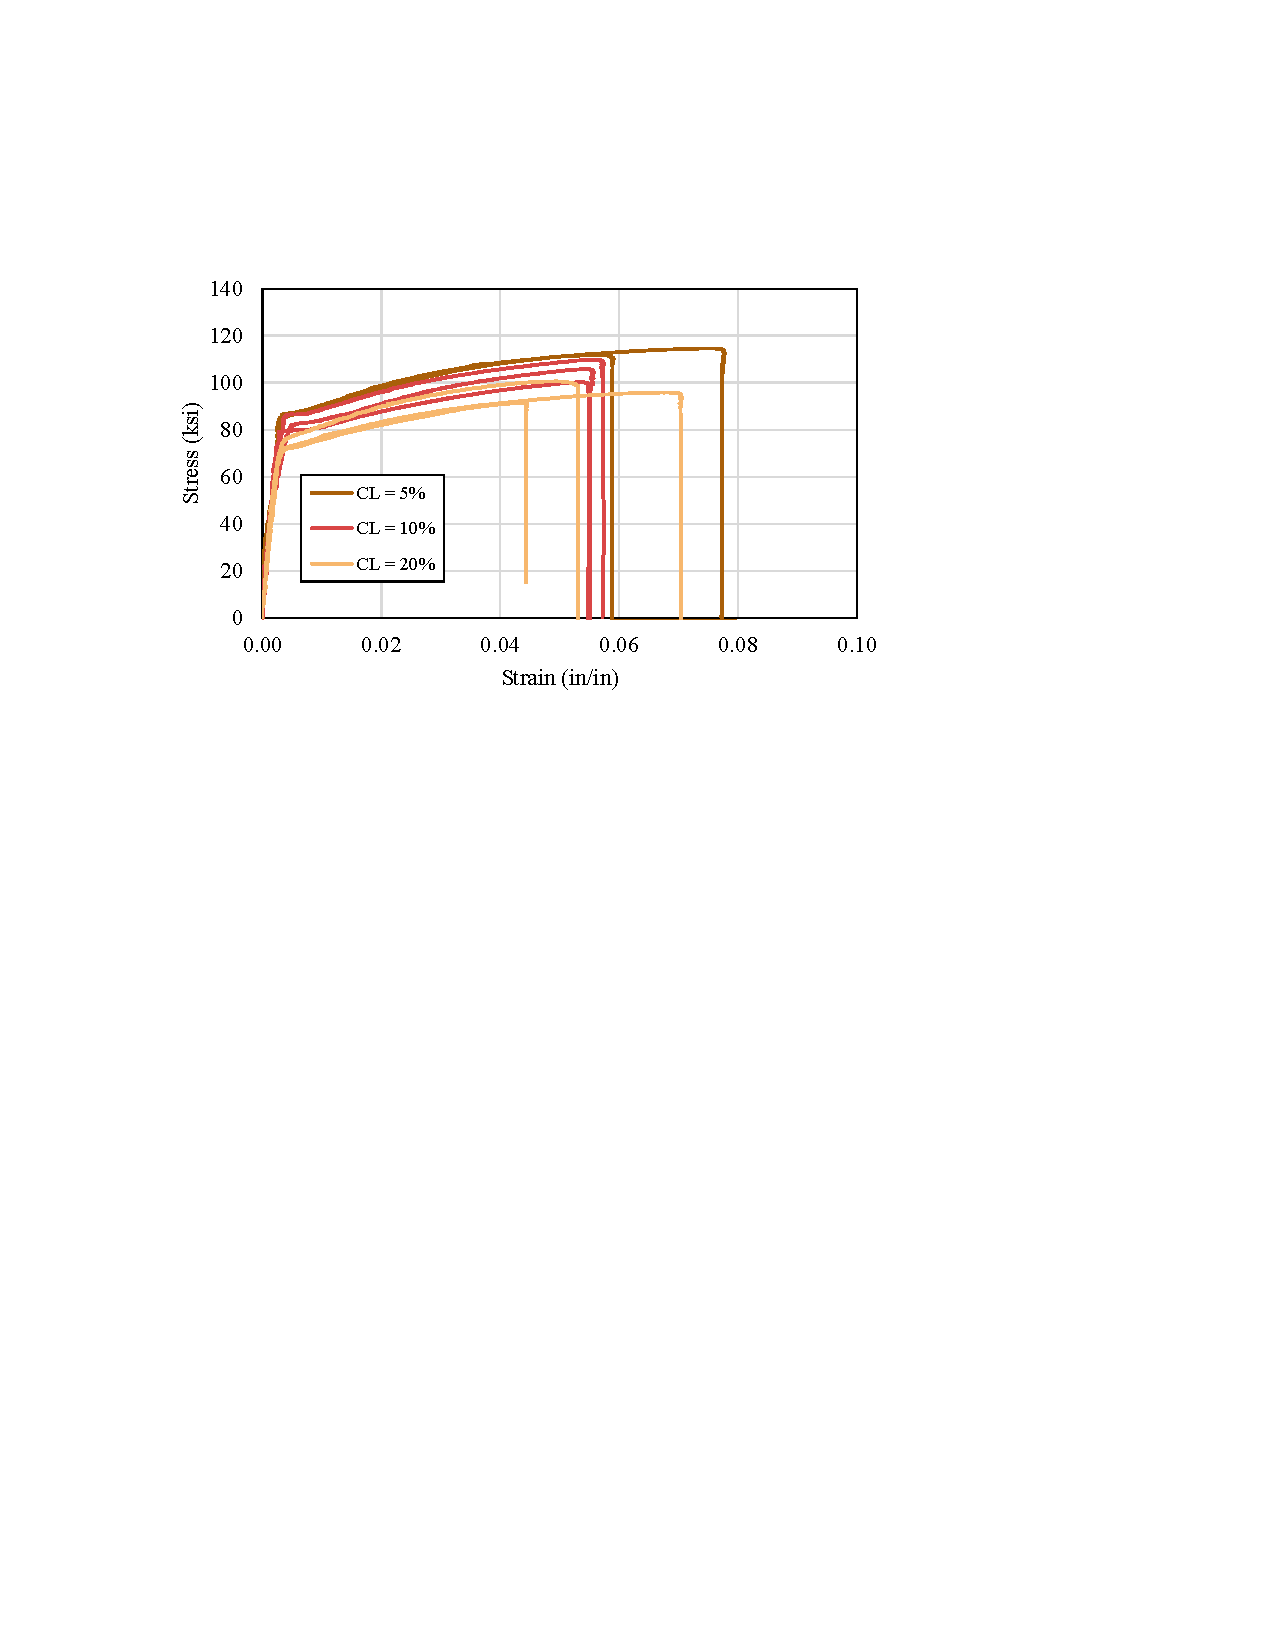
\includegraphics[width=0.7\textwidth]{VAC Thesis 2.0/Chapter-4/figs/TensionTest_results_1.pdf}
	\caption{Tension test results at different corrosion levels}
	\label{fig:TensionTestResults_StressStrain}
\end{figure}

\subsection{Effective Yield Strength as a Function of the Corrosion Level}

Effective yield strength is a mathematical convenience that considers the effect of imperfections in the observed global reduction of the yield strength. \fref{fig:YieldStrength_vs_CL} shows the plot of the effective yield strength ($f_{y,e}$) versus the corrosion level (CL). The results show a linear relationship between the effective yield strength and the corrosion level. This is congruent with other studies performed on other types of steel, such as the study done by Du et al \cite{Du2005}.The apparent reduction in effective yield strength is due to points of concentrated reduction in the geometry of the rebars, which act as stress risers near the area of fracture.

\begin{figure}[htbp]
	\centering
	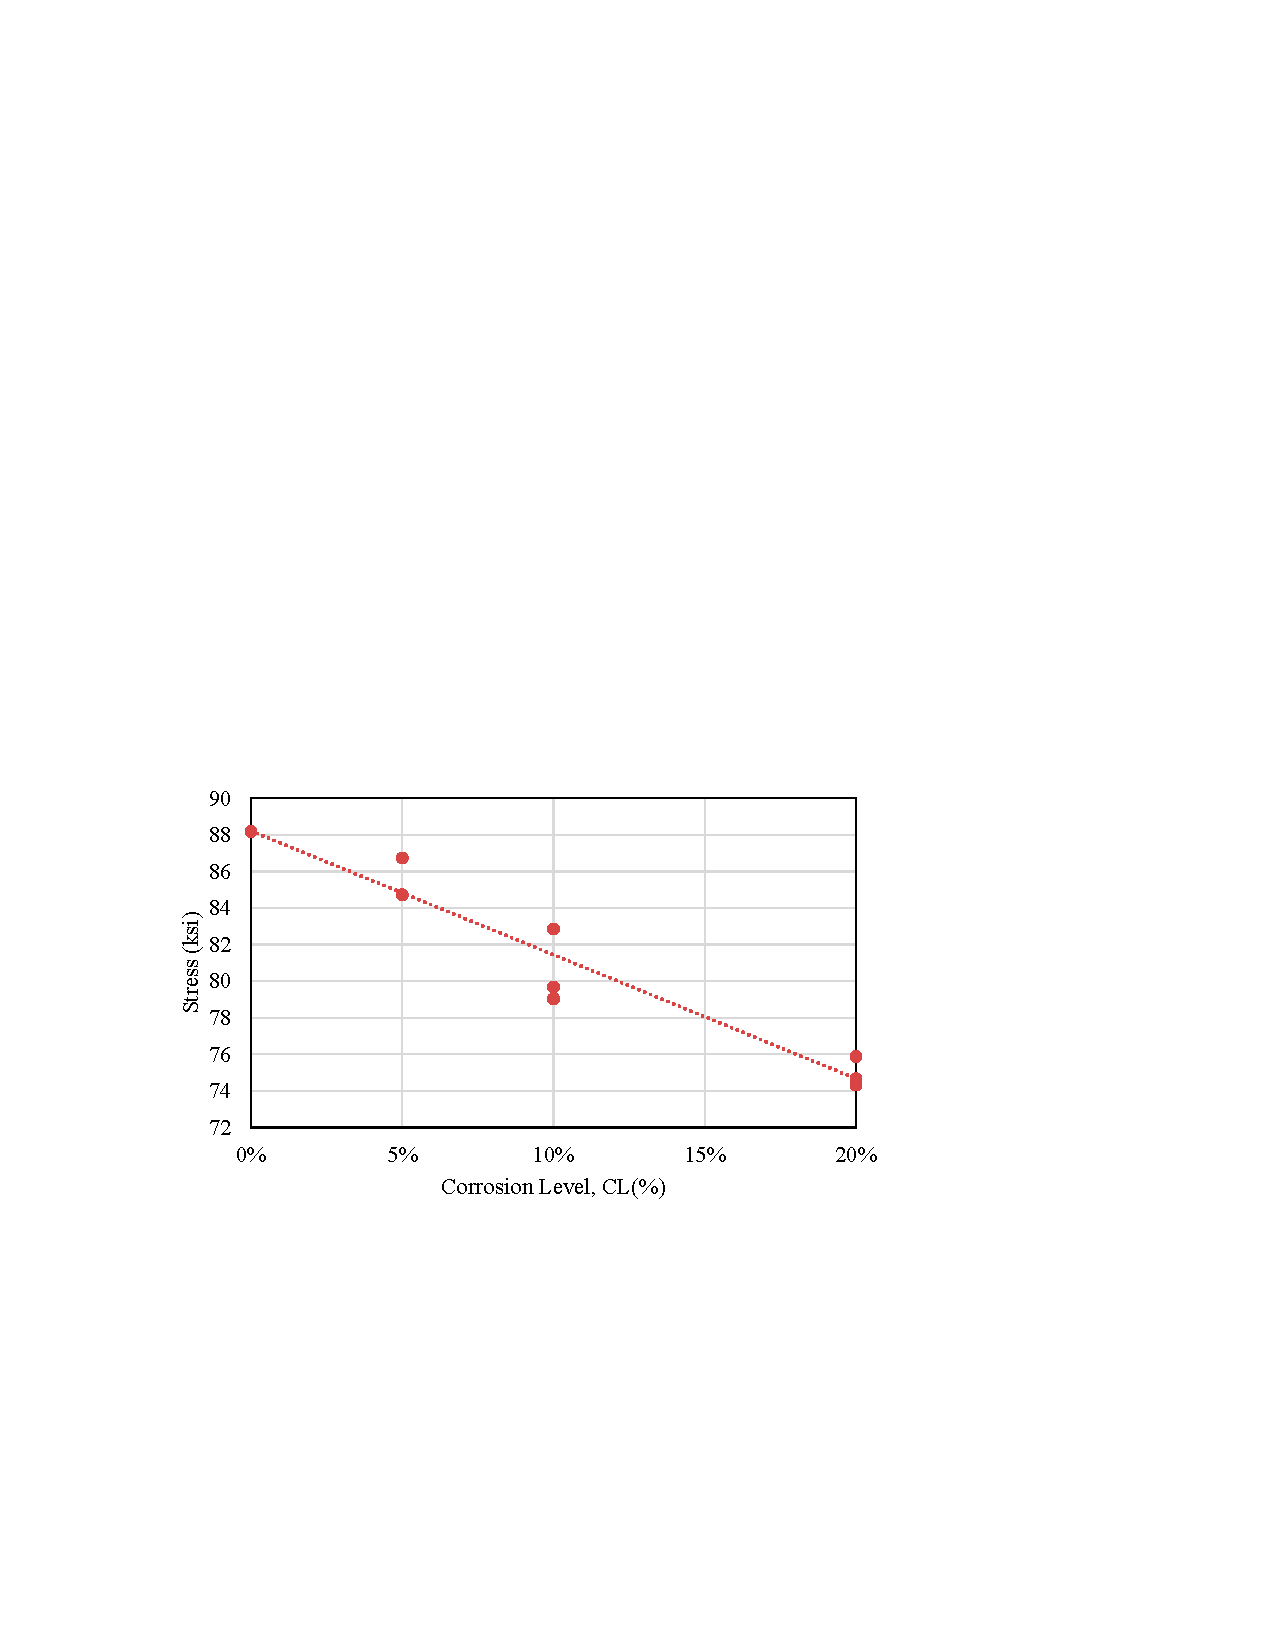
\includegraphics[width=0.7\textwidth]{VAC Thesis 2.0/Chapter-4/figs/TensionTest_results_2.pdf}
	\caption{Yield strength as a function of corrosion level}
	\label{fig:YieldStrength_vs_CL}
\end{figure}

The linear trend observed between the effective yield strength and the corrosion level is expressed as:

\begin{equation}
    f_{y,CL} = f_{y,o}(1-0.0075CL)
    \label{eq.Calderon_Fy_vs_CL}
\end{equation}

The proposed equation is compared to the model proposed by Du et al \cite{Du2005}, replicated here as \eref{eq.Du_Fy_vs_CL_ch4}. 

\begin{equation}
    f_{y,CL} = f_{y,o}(1-0.005CL)
\label{eq.Du_Fy_vs_CL_ch4}
\end{equation}

In \fref{fig:Calderon_vs_Du}, the Du et al model \eref{eq.Du_Fy_vs_CL_ch4} and our proposed model \eref{eq.Calderon_Fy_vs_CL} are compared against the experimental results. Overall it can be observed that the model by Du et al. \cite{Du2005} tends to over-predict the effective yield strength for corroded grade 80 rebars. Therefore, it is possible that there is correlation between the corrosion level and the grade of the rebar; however, the literature on corrosion for different grades of rebar is scarce. 

\begin{figure}[htbp]
	\centering
	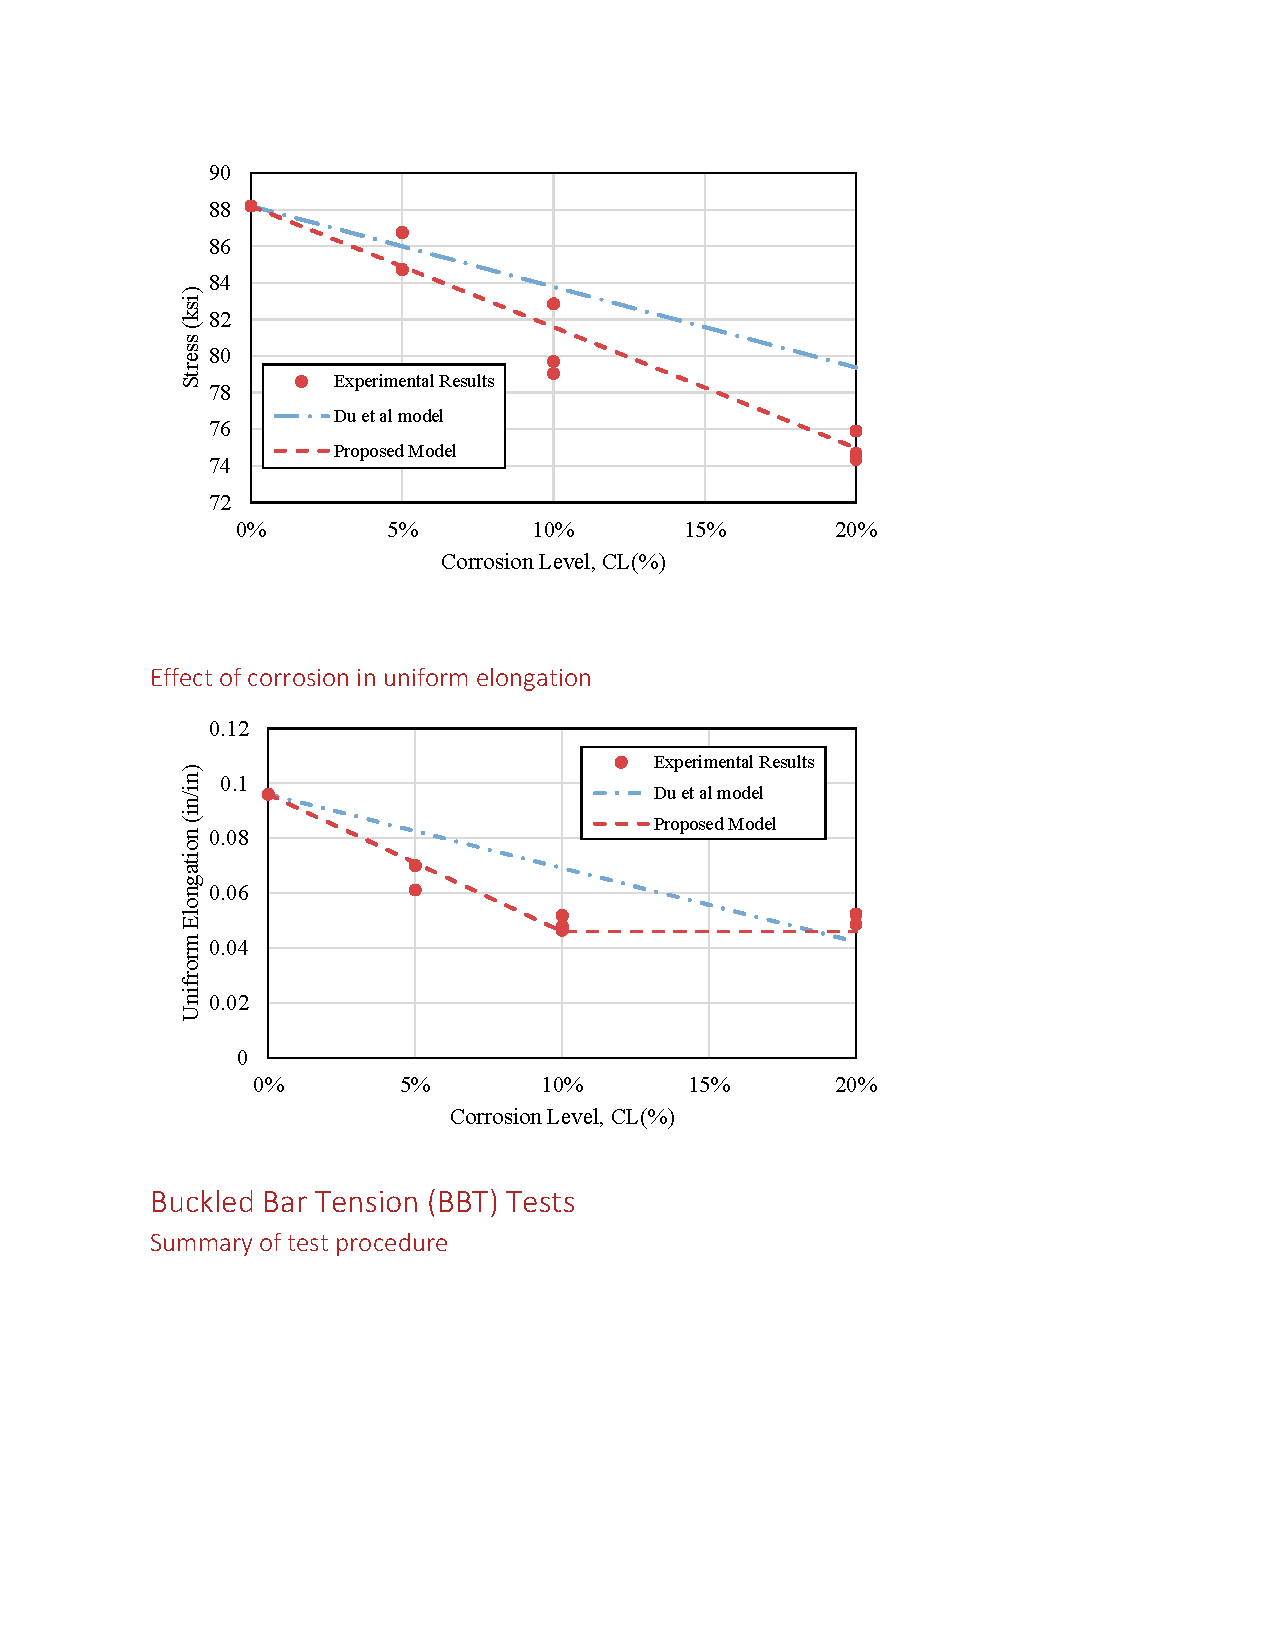
\includegraphics[width=0.7\textwidth]{VAC Thesis 2.0/Chapter-4/figs/TensionTest_results_3_proposedmodel.pdf}
	\caption{Comparison of proposed model and Du et al. model \cite{Du2005} for effective yield strength as a function of corrosion level}
	\label{fig:Calderon_vs_Du}
\end{figure}

\newpage

\subsection{Ultimate Strength as a Function of the Corrosion Level}

A similar trend was observed on the effective ultimate strength of corroded rebars. Past research has shown that the relationship between effective yield strength and effective ultimate strength tend to remain unchanged. In this study, that proved to be the case as well. Replacing, the initial yield strength ($f_y$) with the initial ultimate strength ($f_u$) in \eref{eq.Calderon_Fy_vs_CL}, the effective ultimate strength can be expressed as shown in \eref{eq.Calderon_Fu_vs_CL}. The proposed equation is plotted against the experimental, see \fref{fig:Calderon_ultimate_strength}. The proposed mode predicts the relationship between effective ultimate strength an corrosion level with good agreement with the experimental results.

\begin{equation}
    f_{u,CL} = f_{u,o}(1-0.0075CL)
    \label{eq.Calderon_Fu_vs_CL}
\end{equation}

\begin{figure}[htbp]
	\centering
	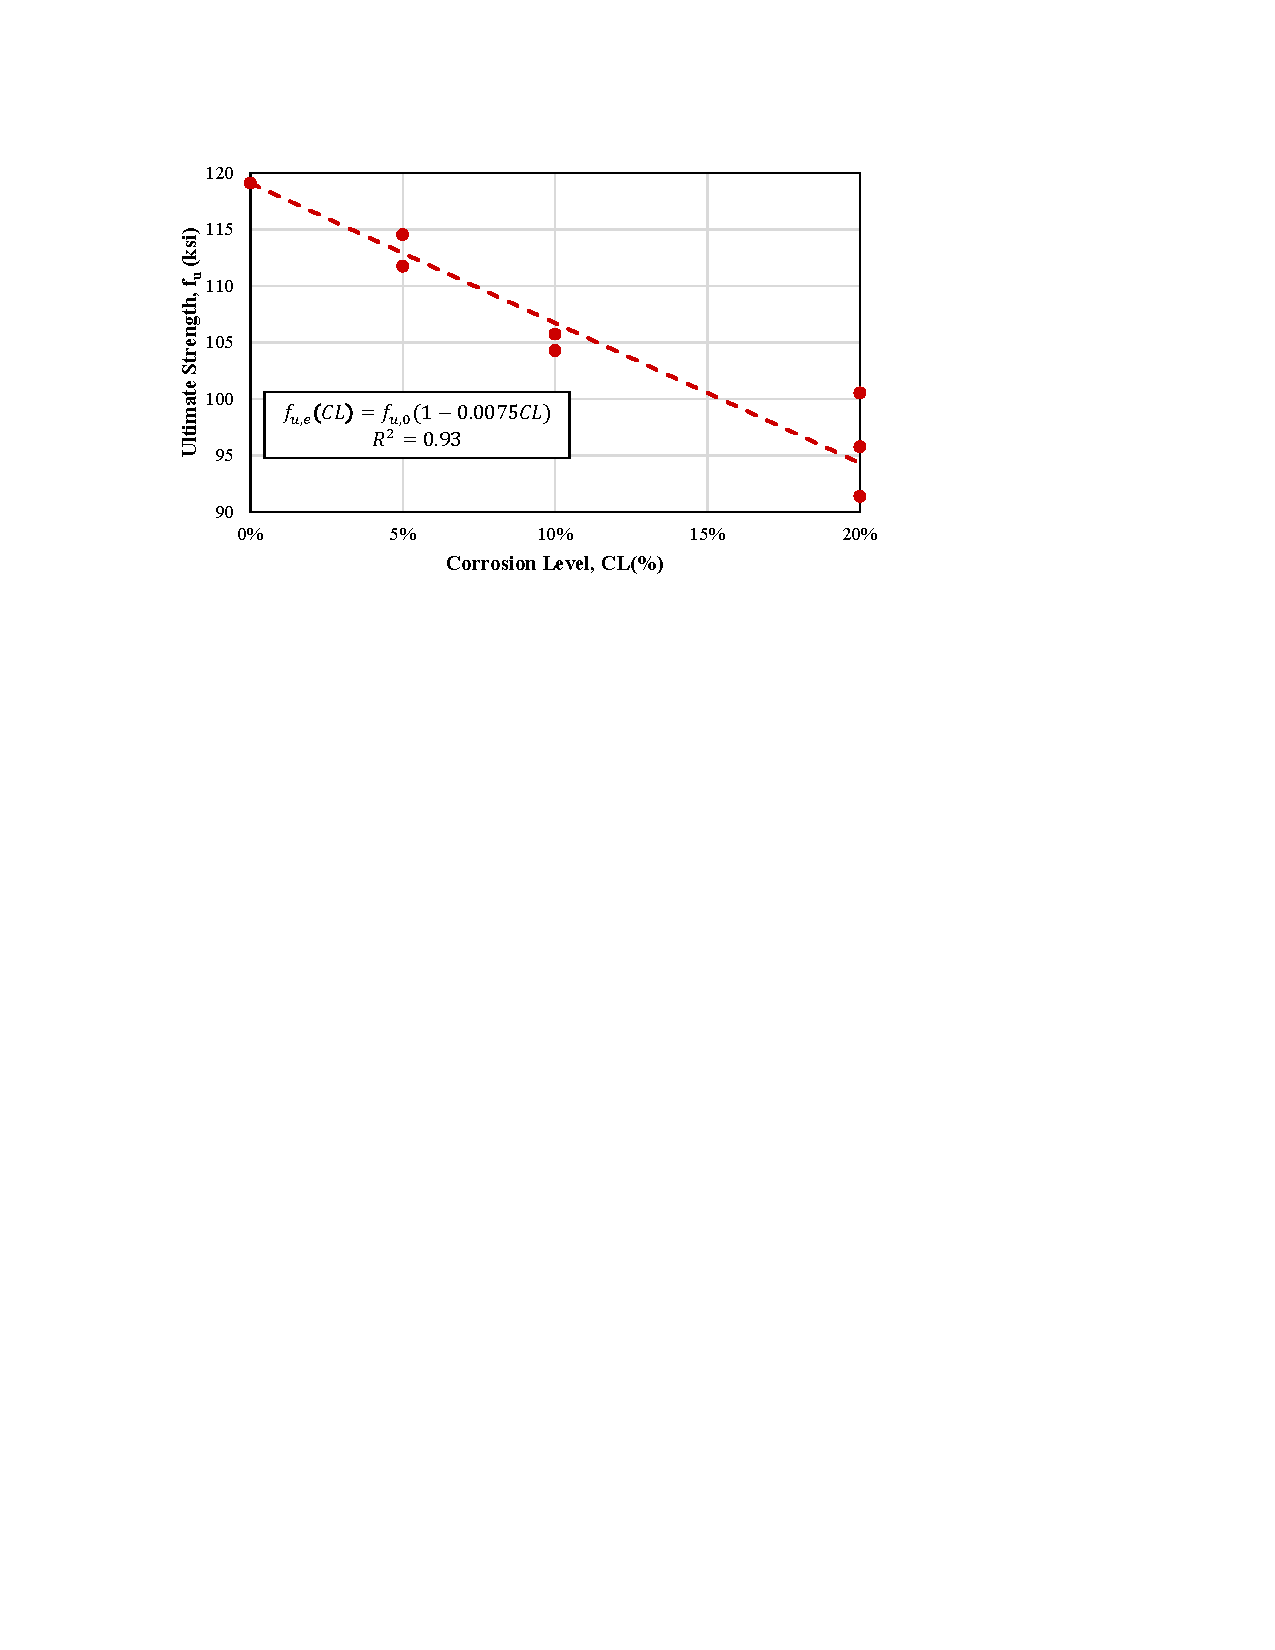
\includegraphics[width=0.7\textwidth]{VAC Thesis 2.0/Chapter-4/figs/TensionTest_results_5_UltimateStrength.pdf}
	\caption{Ultimate strength as a function of corrosion level}
	\label{fig:Calderon_ultimate_strength}
\end{figure}

\subsection{Effect of Corrosion in Uniform Elongation}

Another interesting result was observed on the uniform axial elongation ($\varepsilon_{u}$) property of the corroded rebars. As the rebar corrodes and develops more imperfections on the geometry of the rebar, the uniform axial elongation decreases. The reduction in the uniform axial elongation is linear from the uncorroded state  (CL=0\%) to a corrosion level of 10\%, \fref{fig:UAE_vs_CL} shows this trend more clearly. 

We propose the following model to predict the uniform axial elongation of corroded grade 80 rebars:

For corrosion level between 0\% - 10\%
\begin{equation}
    \varepsilon_{CL} = \varepsilon_{o}-0.05CL
    \label{eq.Calderon_UAE_vs_CL}
\end{equation}

For corrosion level larger than 10\%

\begin{equation}
    \varepsilon_{CL} = 0.045
    \label{eq.Calderon_UAE_vs_CL20}
\end{equation}

\begin{figure}[htbp]
	\centering
	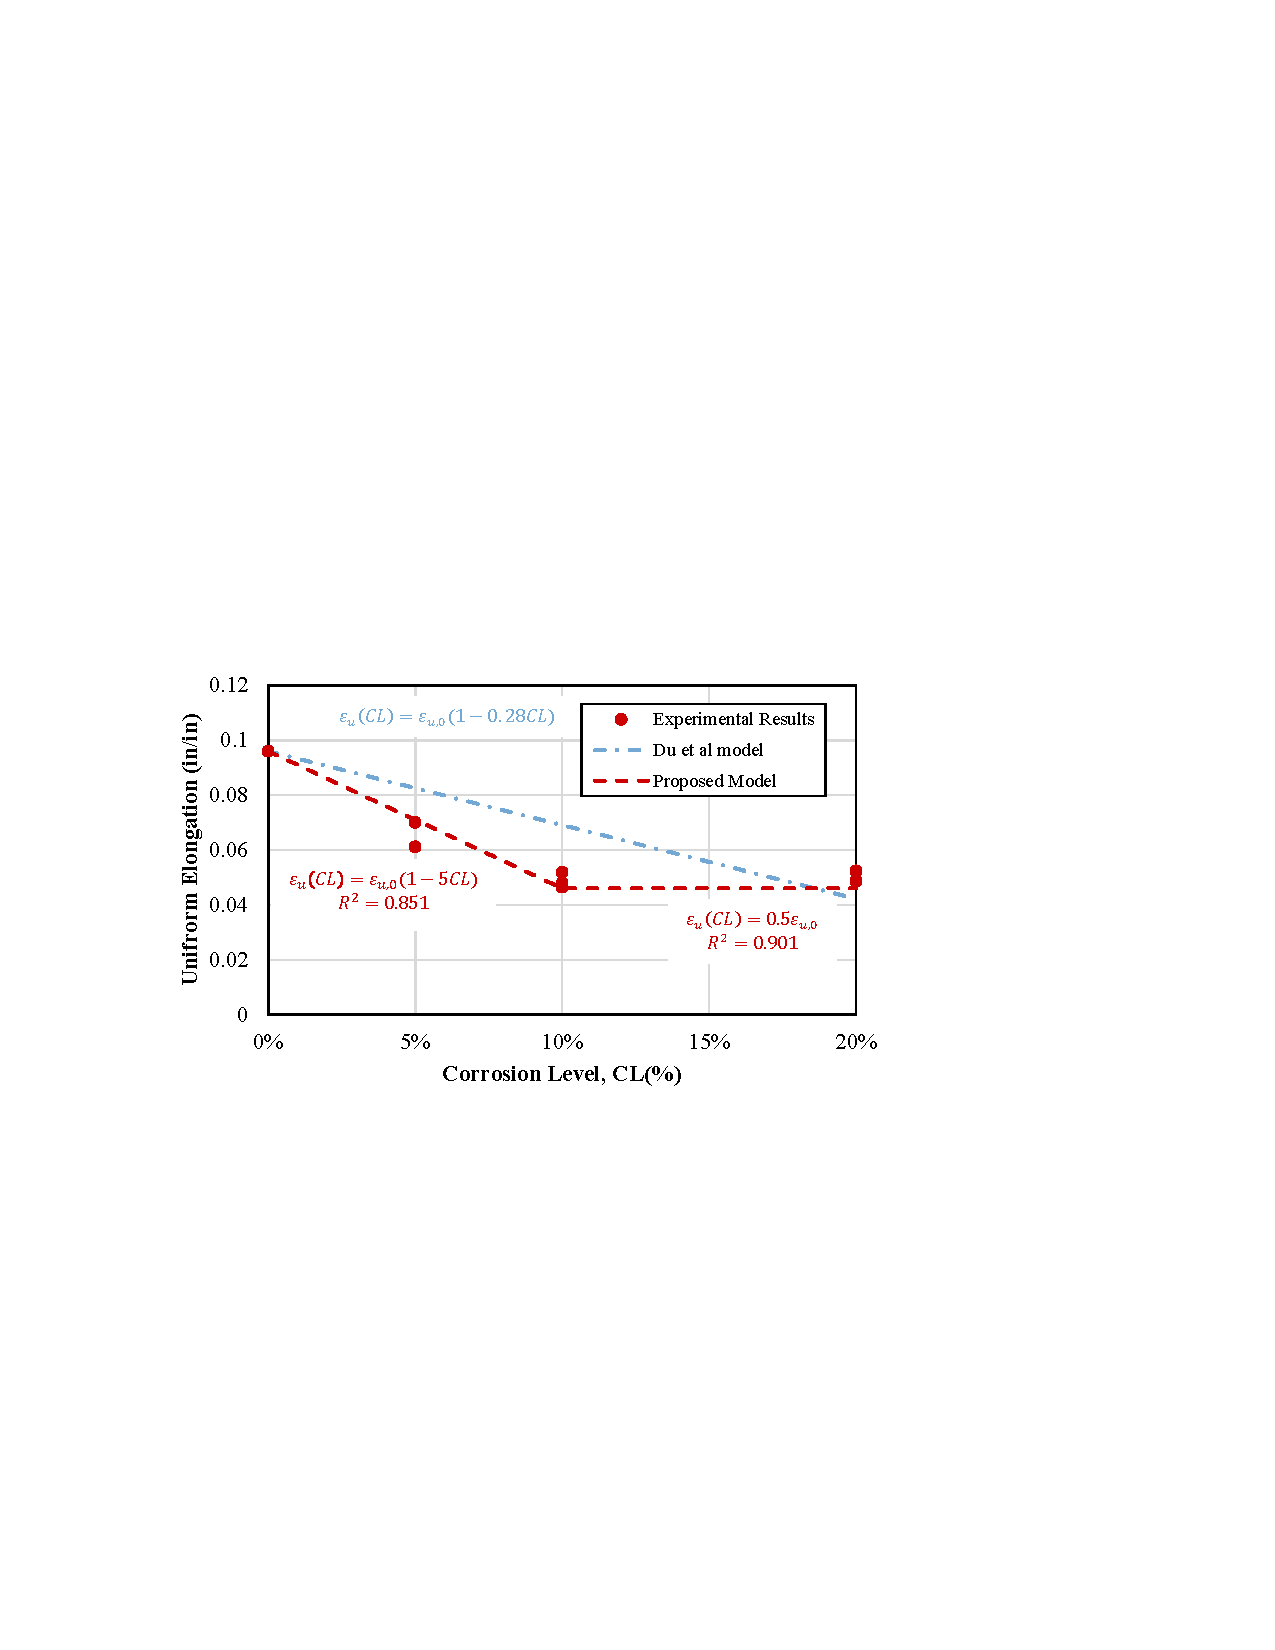
\includegraphics[width=0.7\textwidth]{VAC Thesis 2.0/Chapter-4/figs/TensionTest_results_4_proposedmodel.pdf}
	\caption{Comparison of proposed model and Du et al. model \cite{Du2005} for uniform axial elongation ($\varepsilon_u$) as a function of the corrosion level (CL)}
	\label{fig:UAE_vs_CL}
\end{figure}

\section{Buckled Bar Tension (BBT) Tests}
\subsection{Summary of BBT Procedure}

The buckled bar tension test is shown in \fref{fig:BBT_Test_Summary} and consists of: 1) Loading the bar with the LED markers in the UTM machine, 2) Compressing the bars to a prescribed level of bending strain, 3) Loading the rebar in tension, and  4) Recording the type of fracture: Ductile or Brittle, see \fref{fig:bbt_brittle_vs_duc}. 

\begin{figure}[htbp]
	\centering
	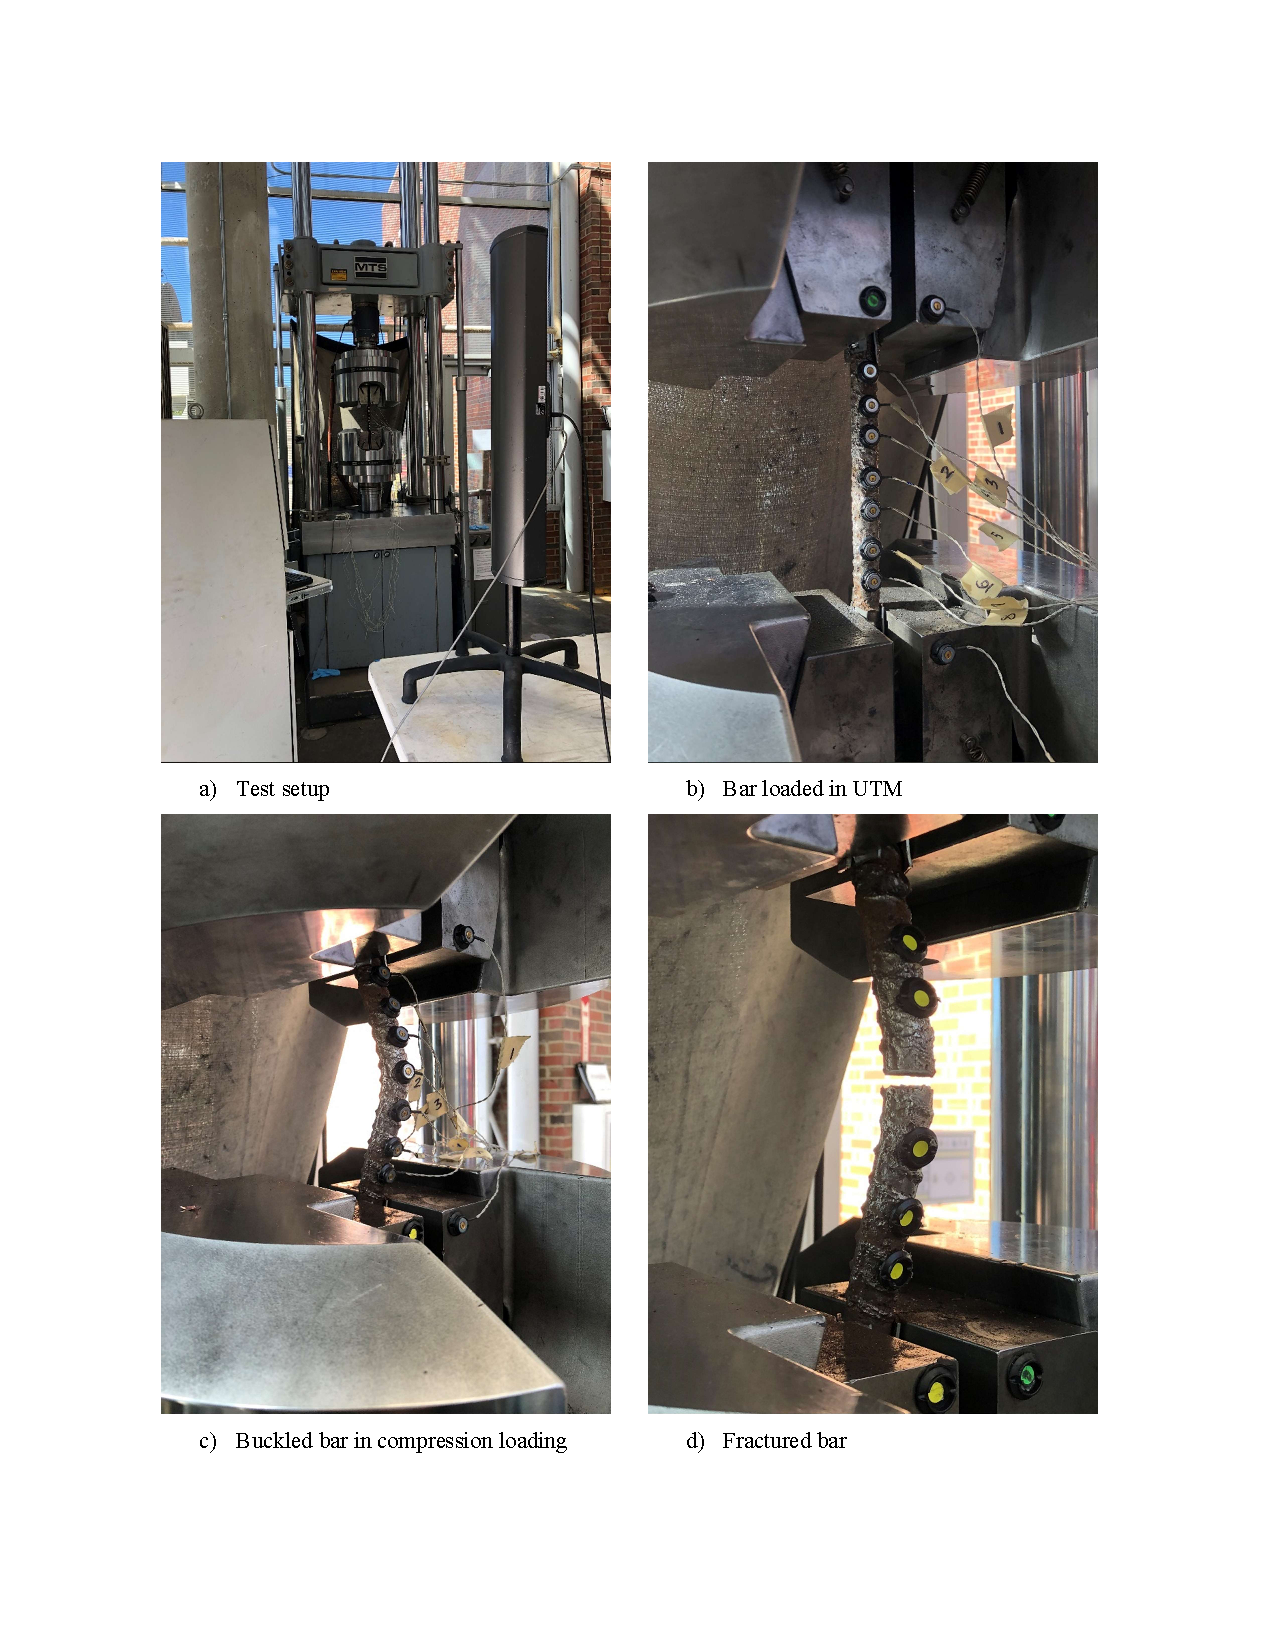
\includegraphics[width=0.7\textwidth]{VAC Thesis 2.0/Chapter-4/figs/BBT Procedure.pdf}
	\caption{General procedure of buckled bar tension (BBT) test}
	\label{fig:BBT_Test_Summary}
\end{figure}

\begin{figure}[htbp]
	\centering
    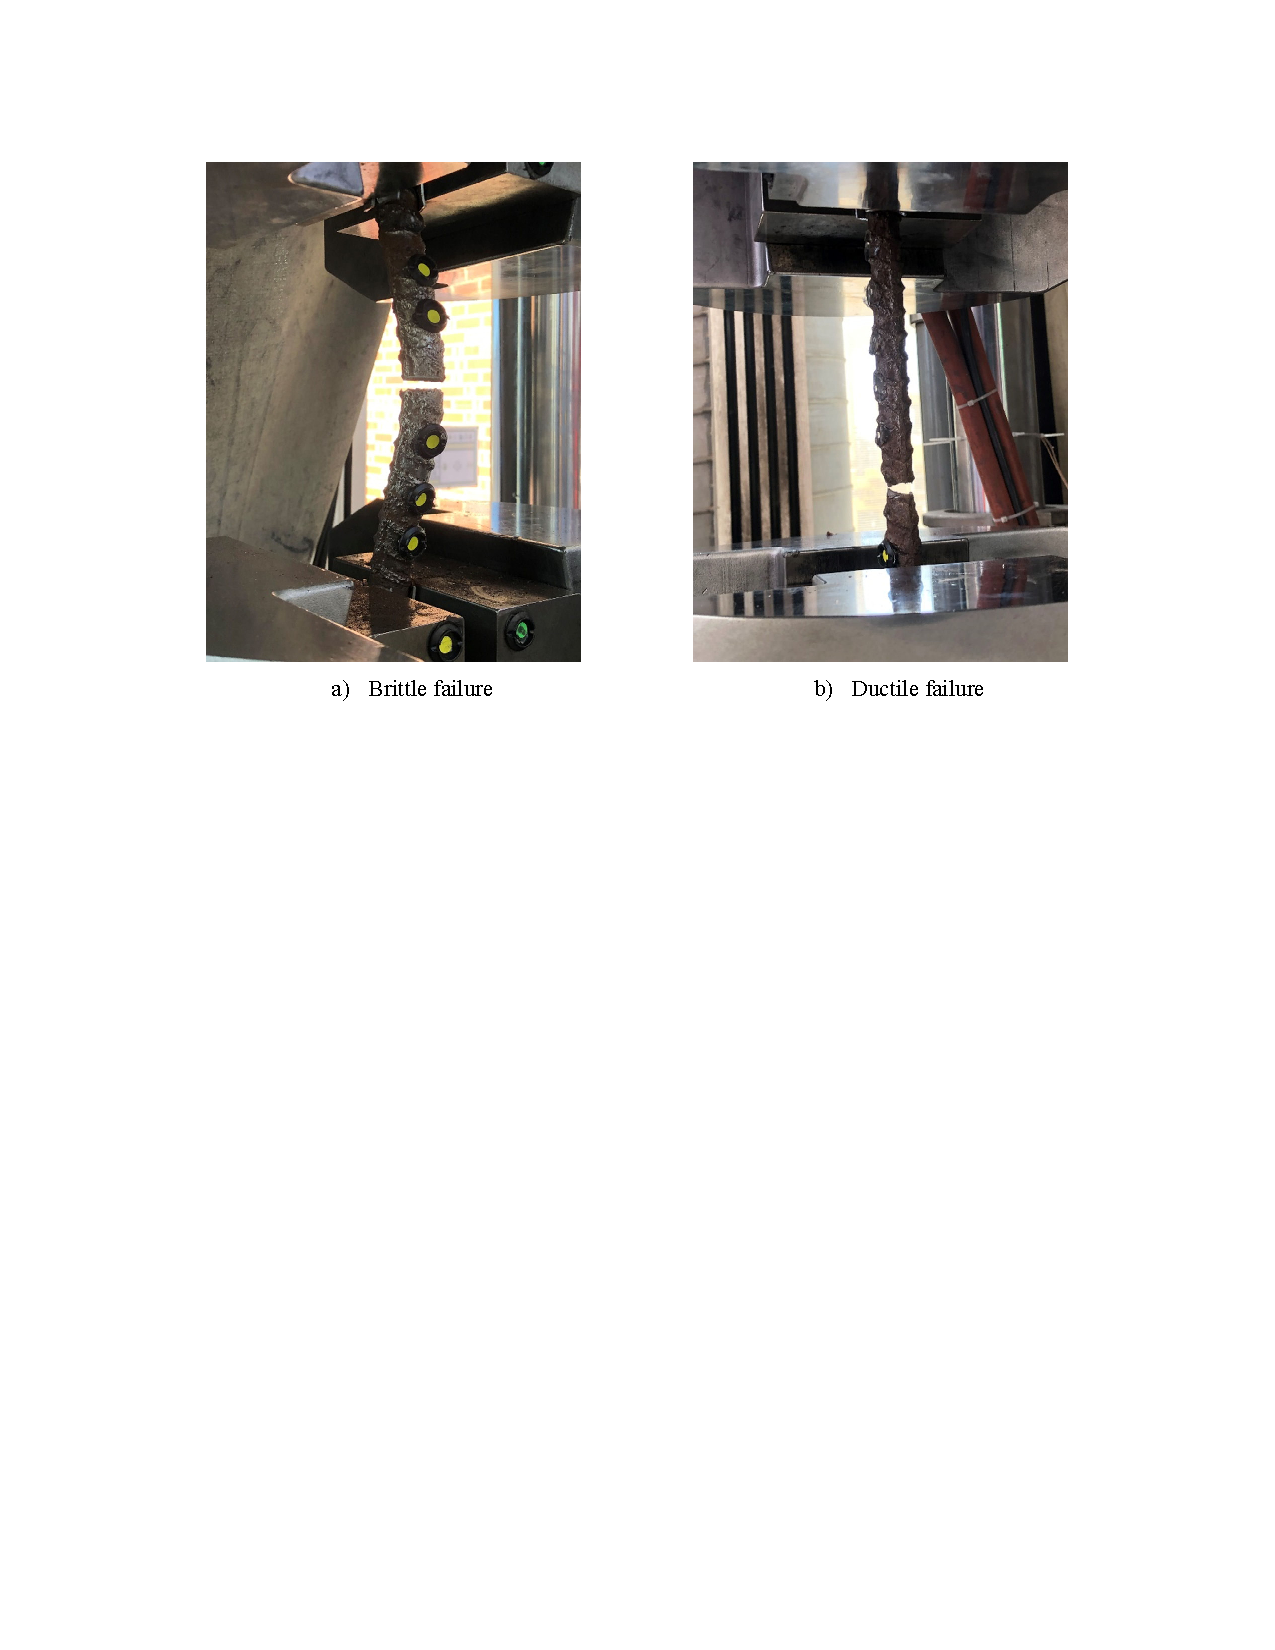
\includegraphics[width=0.7\textwidth]{VAC Thesis 2.0/Chapter-4/figs/BBT_Brittle_vs_Ductile_fracture.pdf}
	\caption{Type of failures in BBT tests}
	\label{fig:bbt_brittle_vs_duc}
\end{figure}

The data obtained from the BBT test was then processed and two parameters were obtained: 1) the critical bending strain, based on the curvature, and 2) the maximum uniform axial deformation is obtained from the stress strain curve. These two values are obtained as shown in \fref{fig:bendingstrain}. In the case of brittle failure, if the bar does not elongate compared to its original length, the uniform axial elongation is assigned a value of zero.

\begin{figure}[htbp]
	\centering
	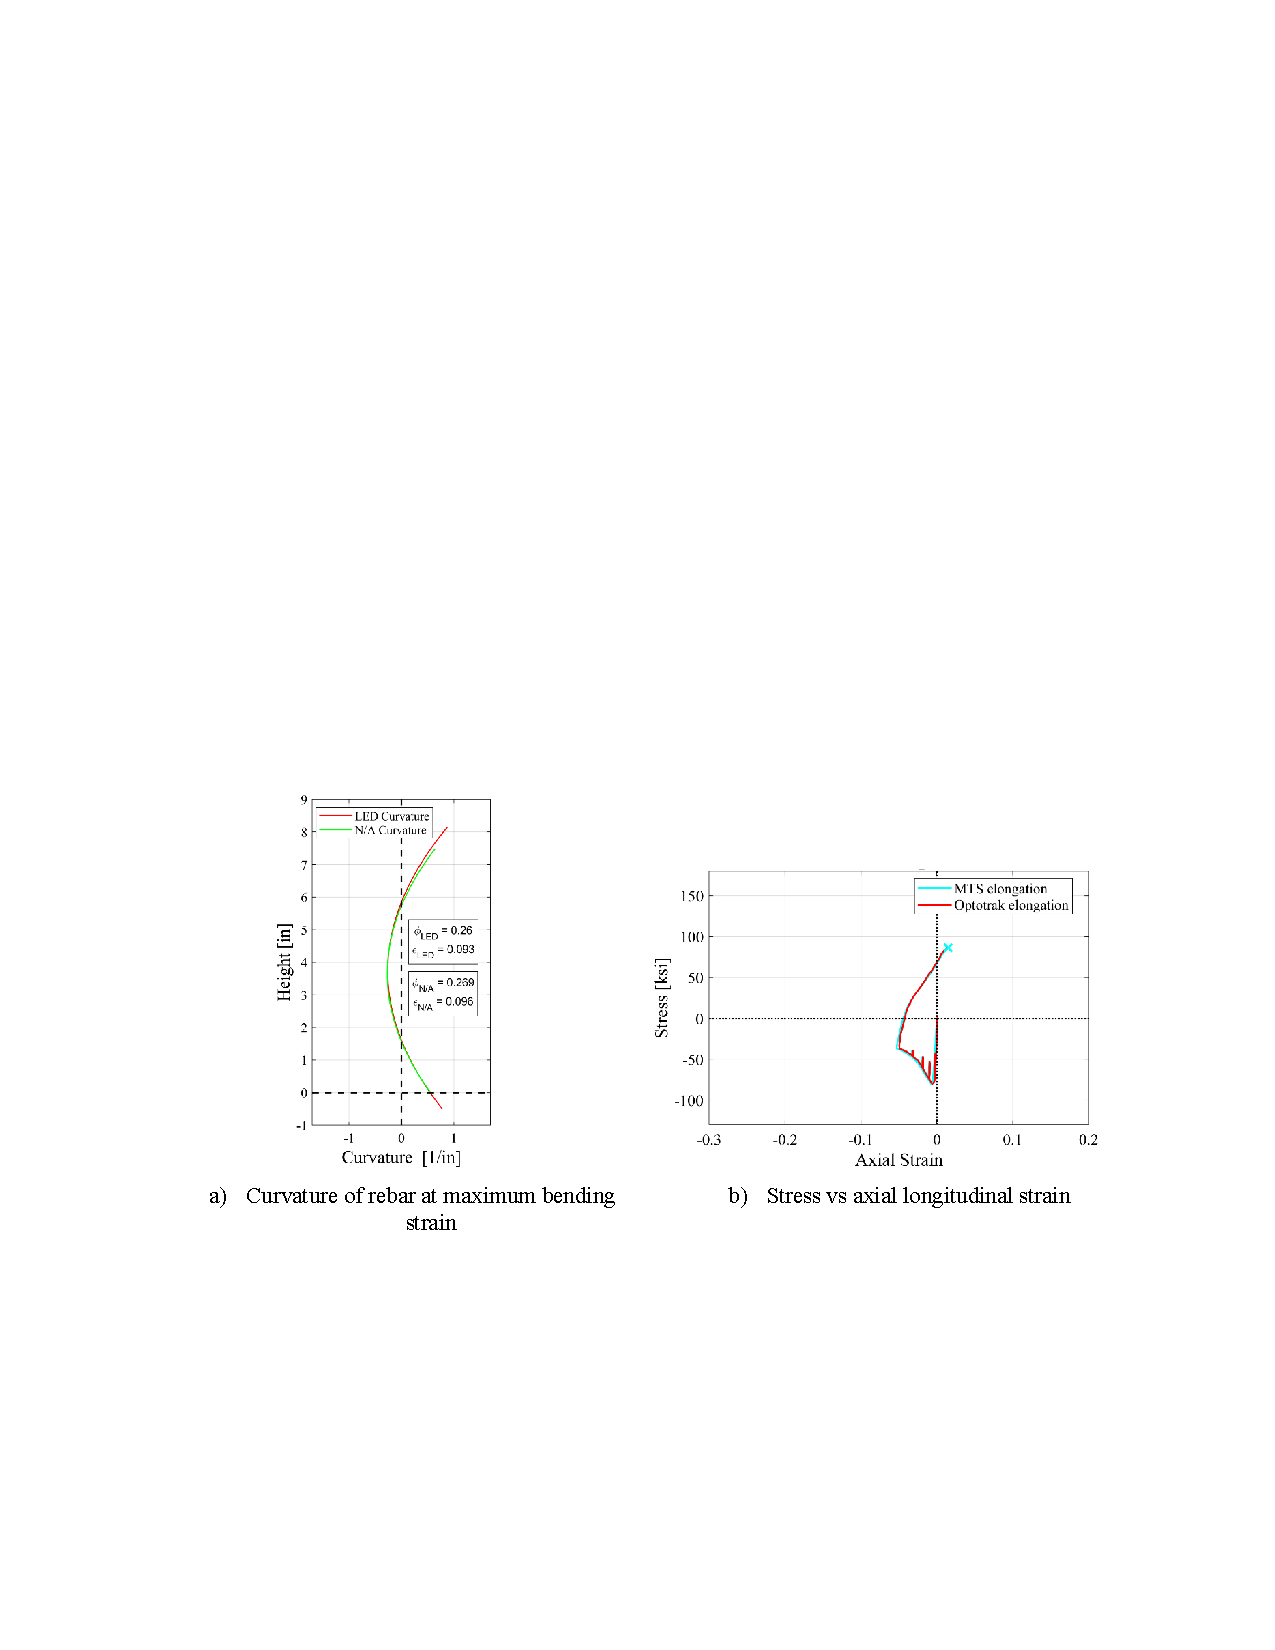
\includegraphics[width=1\textwidth]{VAC Thesis 2.0/Chapter-4/figs/BBT_curvature.pdf}
	\caption{Obtaining critical bending strain}
	\label{fig:bendingstrain}
\end{figure}

\subsection{Effect of Corrosion in Critical Bending Strain}

The buckled bar tension test was applied to rebars with varying levels of corrosion ranging from 0\% - 20\%. For each corrosion level a total of 6 BBT tests were performed. From the BBT tests data, the bending strain versus the uniform axial elongation is plotted. As shown in \fref{fig:BBT_strains} the critical bending strain is defined as the bending strain at which, after pulling the buckled bar in  tension, the uniform axial elongation is zero. This is the case for brittle failures and is higher for ductile failures. The process described previously is repeated for each corrosion level. The bending strain versus uniform axial elongation for each corrosion level, along with the critical bending strain at a given corrosion level ($\varepsilon_{b,CL}$ are shown in  \fref{fig:BBT_strains}. The benchmark value of pristine bars (CL=0\%) was obtained from the study by Barcley et al \cite{Barcley2018}. In \fref{fig:eb_vs_CL} it is noticeable that as corrosion level increases the maximum bending strain reduces. There is also a significant reduction in the uniform axial elongation for the ductile failures at all corrosion levels.

\begin{figure}[htbp]
	\centering
	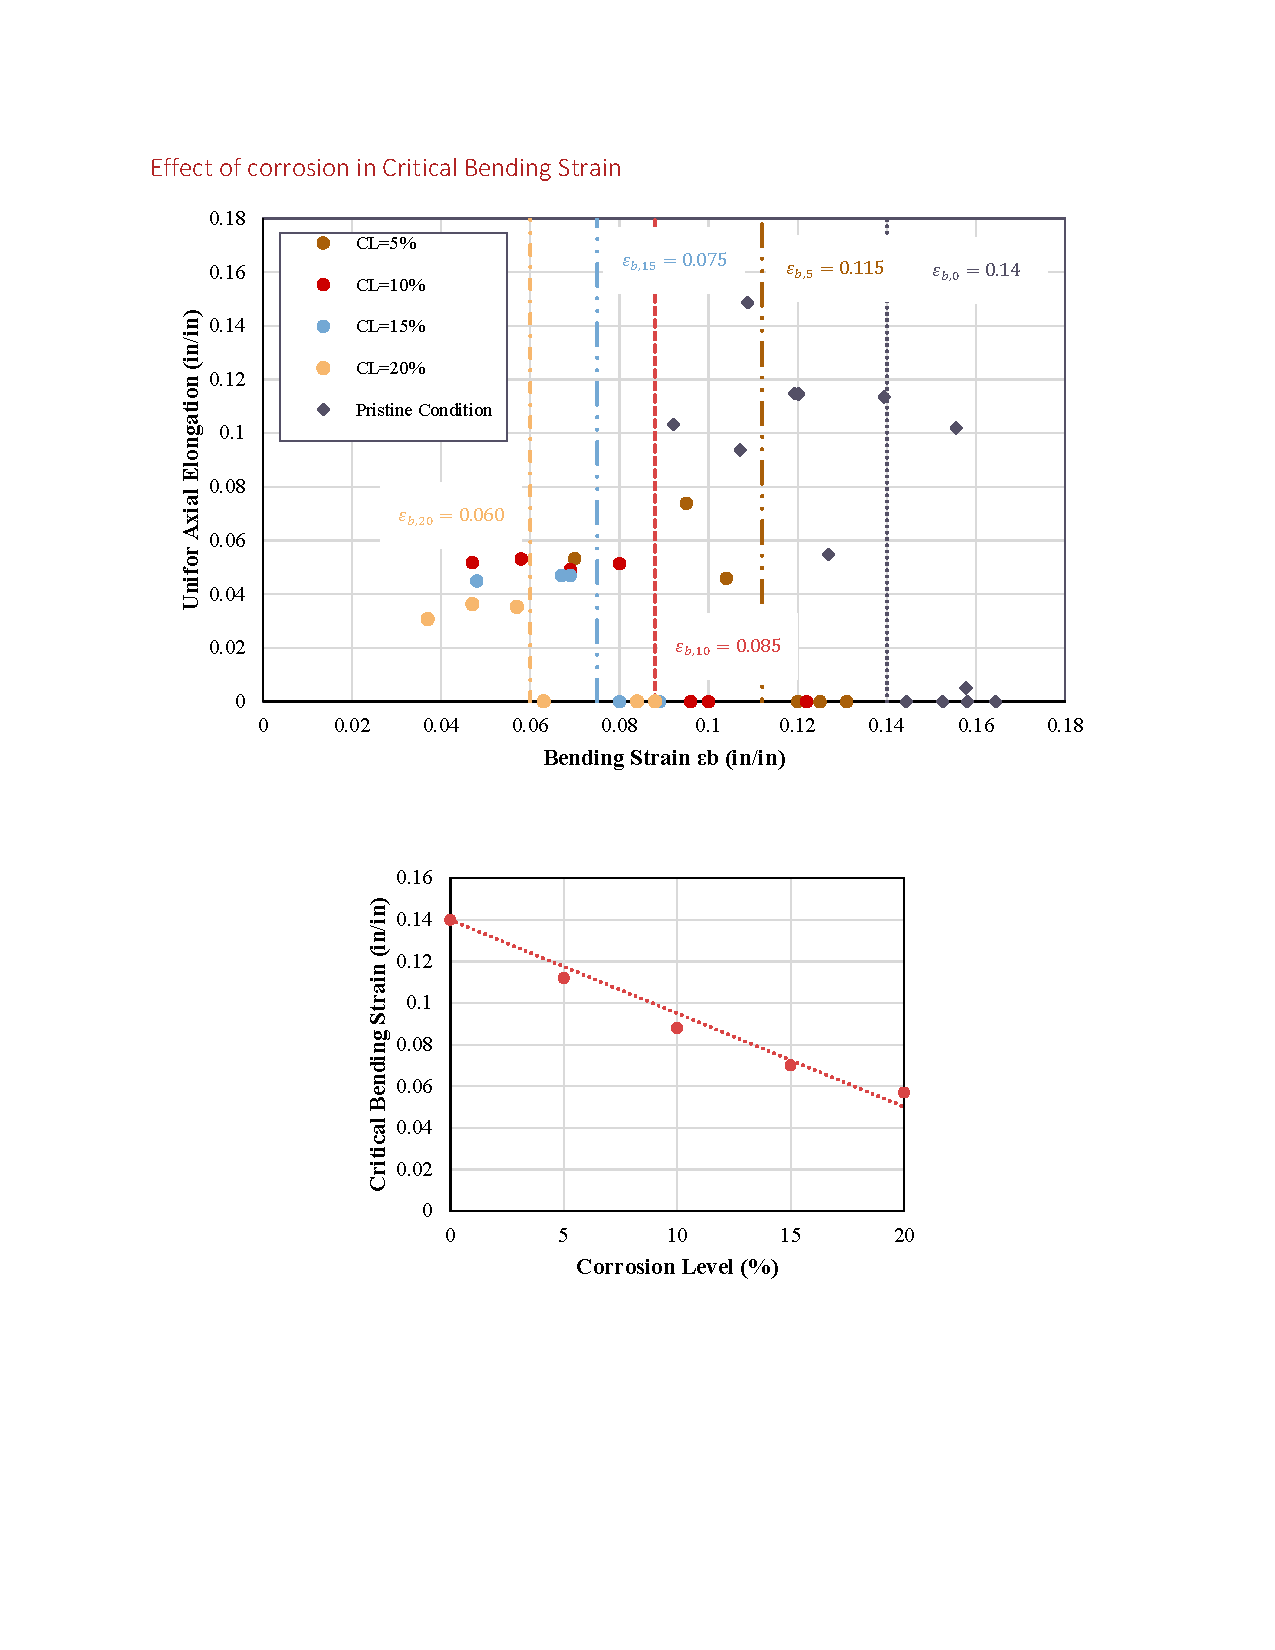
\includegraphics[width=0.95\textwidth]{VAC Thesis 2.0/Chapter-4/figs/BBT_results_.pdf}
	\caption{Bending strain at different corrosion levels}
	\label{fig:BBT_strains}
\end{figure}

Plotting the critical bending strain versus the corrosion level as shown in \fref{fig:eb_vs_CL}, it can be seen that there is a linear relationship between both variables, similar to the results observed in the tension tests. The relationship between corrosion level and critical bending strain ($\varepsilon_{b}$) using linear regression can be expressed as shown below in \eref{eq.Calderon_eb_vs_CL}.

\begin{equation}
    \varepsilon_{b}(CL) = \varepsilon_{o}-0.0045CL
    \label{eq.Calderon_eb_vs_CL}
\end{equation}

It is interesting to notice the sharp drop in critical bending strain capacity as corrosion increases. For CL=5\%, There is a drop of about 20\%; for CL=10\%, the change is 60\% of the pristine condition; and for CL=20\%, that difference is more than 140\% decrease in the critical bending strain. These results indicate that there is a reduction in the ultimate capacity of rebars as they corrode. Based on these results and previous tests performed on corroded RC beams reported by Du et al \cite{Du2005}, and on RC columns as shown by Ma et al \cite{Ma2012} and Meda et al \cite{Meda2014}. A limiting value of corrosion levele for serviceability is recommended at CL=10\%.

\begin{figure}[htbp]
	\centering
	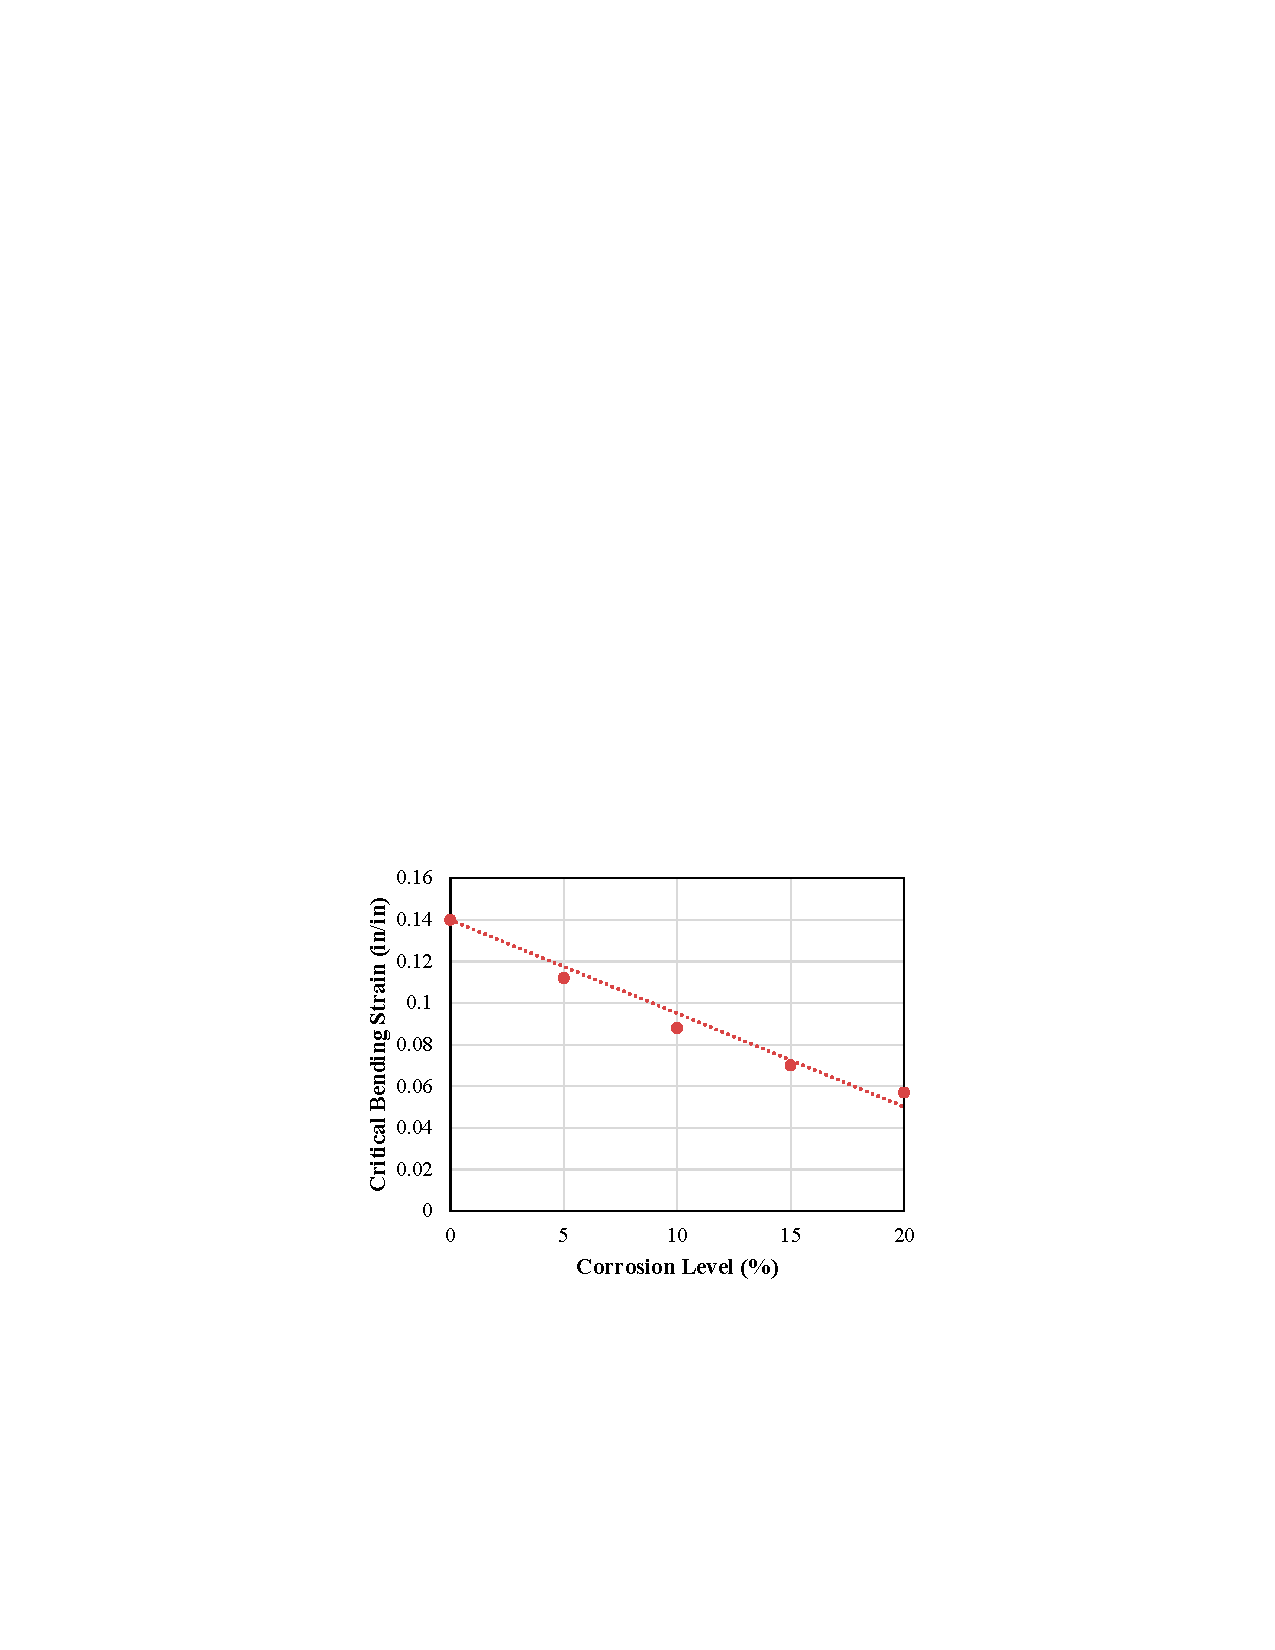
\includegraphics[width=0.6\textwidth]{VAC Thesis 2.0/Chapter-4/figs/BBT_results_summary.pdf}
	\caption{Maximum bending strain as a function of corrosion level}
	\label{fig:eb_vs_CL}
\end{figure}

\subsection{Effect of Corrosion at the Micro-structural Level}

To study if there was any change in the microstructural behavior of the rebars as they corroded and explore if the chlorides induced fracture in the rebars at the point of fracture, the rebars' fracture surfaces were observed under a Variable Pressure Scanning Electron Microscope (VPSEM). Fracture surfaces from ductile and brittle failures were obtained at ductility levels of 5\%-20\%.

\textbf{Fractography of BBT test specimens fracture surfaces}

 As previously observed in \fref{fig:bbt_brittle_vs_duc}, at the macro level brittle fractures typically consist of flat fracture surface, and in ductile fractures, there is necking and rougher edges along the fracture surface. The observations at the macro level translate into similar observations at the microstructural level. To analyze the images obtained from the Scanning Electron Microscope (SEM), it is important to understand what brittle and ductile fractures in metals look like under the SEM. \fref{fig:fractography101} summarizes the typical features for brittle fractures and ductile fractures. Brittle fractures present features that tend to promote flat surfaces. The two main types of brittle fractures are granular and cleavage. Ductile fractures, on the other hand, have dimple features, which is due to the extension of the fracture surface at the point where atomic bonds are broken.
 
\begin{figure}[htbp]
	\centering
	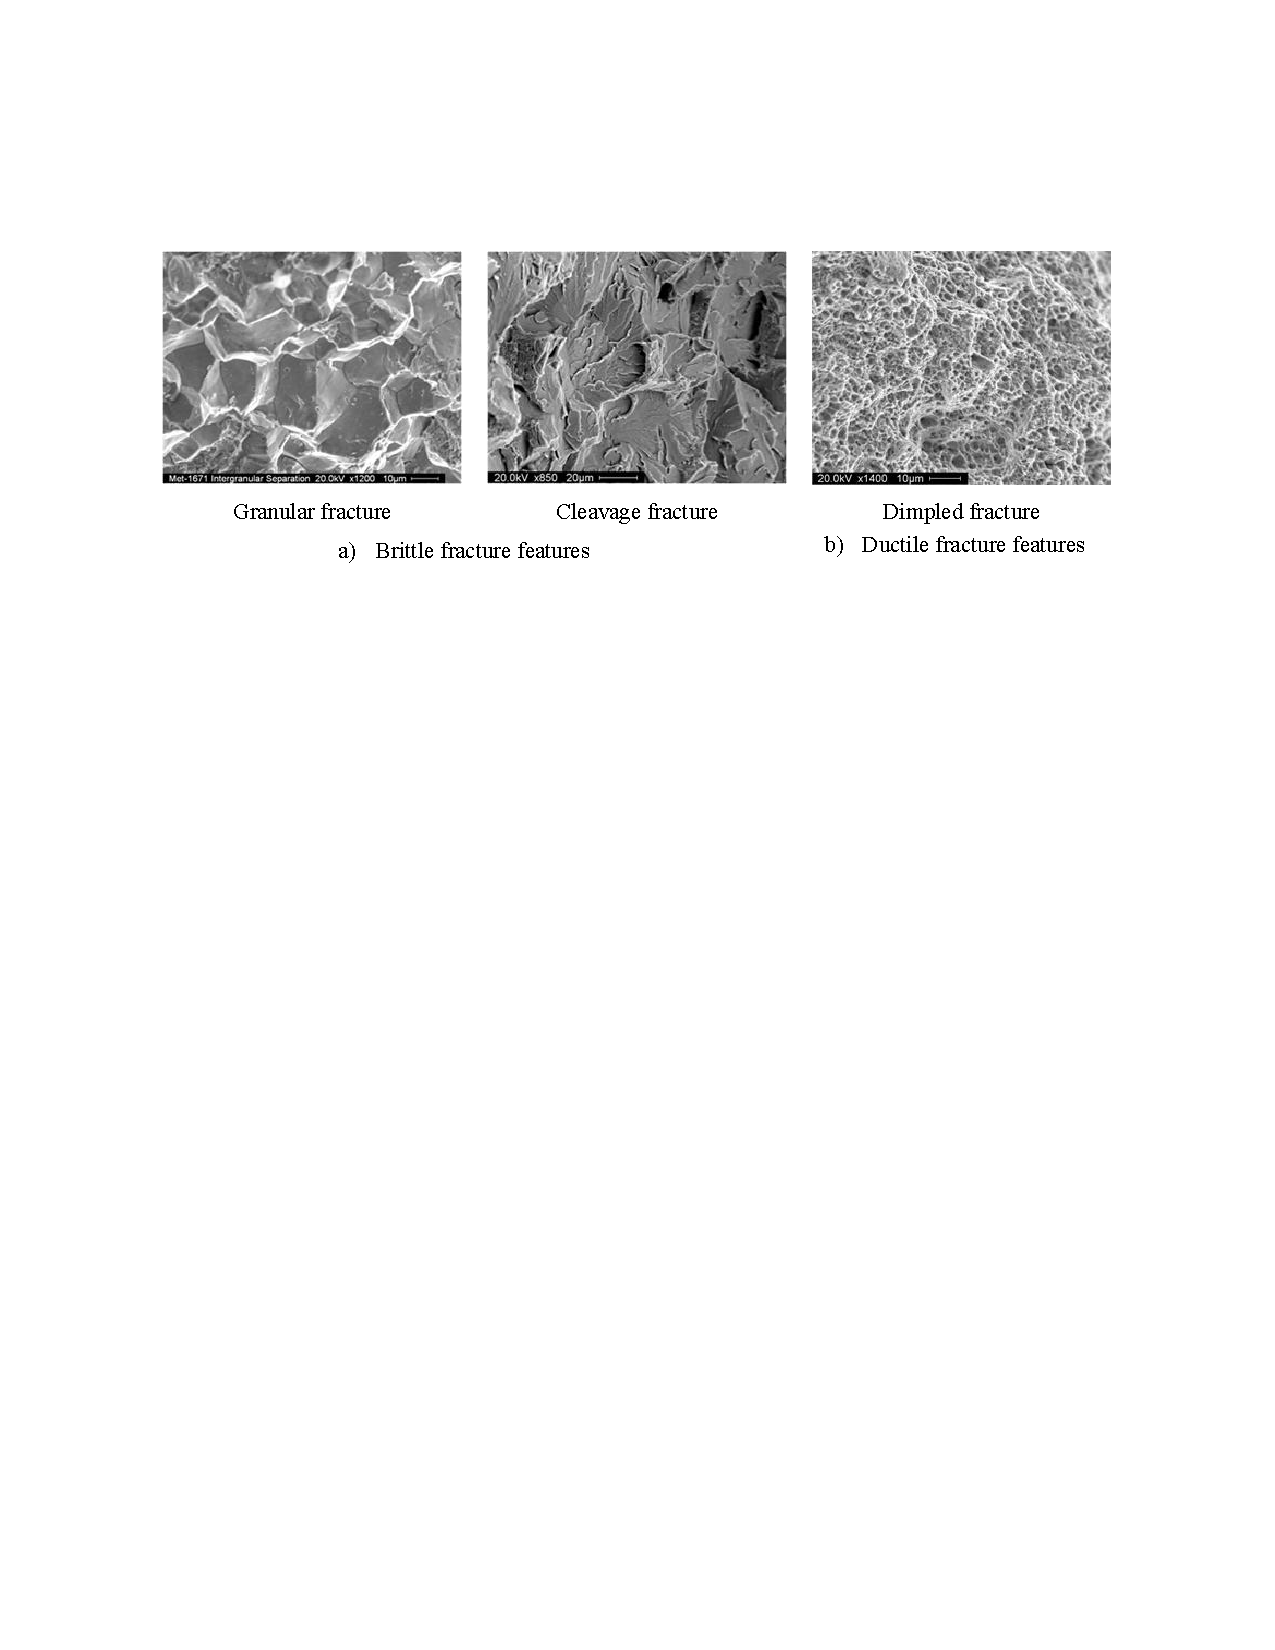
\includegraphics[width=0.825\textwidth]{VAC Thesis 2.0/Chapter-4/figs/FractographyBasics_101.pdf}
	\caption{Basic features analysis of fracture surfaces in metals}
	\label{fig:fractography101}
\end{figure}

\fref{fig:FractureSurfaces} summarizes the observations performed on the fracture surfaces. While VPSEM images were obtained for each corrosion level, no substantial differences for brittle and ductile samples was observed as the corrosion level increased. Therefore, the observations performed on the CL=10\% samples are shown here as representative of all the observations. The methodology of the observations was in such a way that differences between different sectors of the fracture provided comparison points.  \fref{fig:FractureSurfaces} shows three main sectors: 1) the point of initiation of fracture, 2) the midpoint, and 3) the extreme fiber opposite of the initiation of fracture. In all cases, the point of initiation of fracture occurred where the extreme fiber was subjected to tension while being compressed.

Comparing the images obtained for the brittle and ductile response in \fref{fig:FractureSurfaces}, we can make the following observations. 1) At the point of initiation of fracture for the brittle and ductile surfaces, there is no difference in the behavior of the fracture surfaces observed, indicating that the point of initiation of fracture is always brittle in nature. This can be seen in the presence of flat surfaces. 2) At the midpoint we start to observe some differences in the brittle sample. Flat surfaces are still observed, but for the ductile sample, a mixture of flat surfaces and dimples typical of ductile surfaces are observed.This mixture of responses is similar to SEM observations of fracture surfaces of fatigue fractures. 3) At the extreme fiber point, the difference between ductile and brittle is more prominent, since the ductile response has a predominant presence of dimples and the brittle response still shows flat surfaces. These results tell us the different mechanisms that occur between the brittle and ductile response, and correlate well with the observed behavior of the BBT tests.

\begin{figure}[htbp]
	\centering
	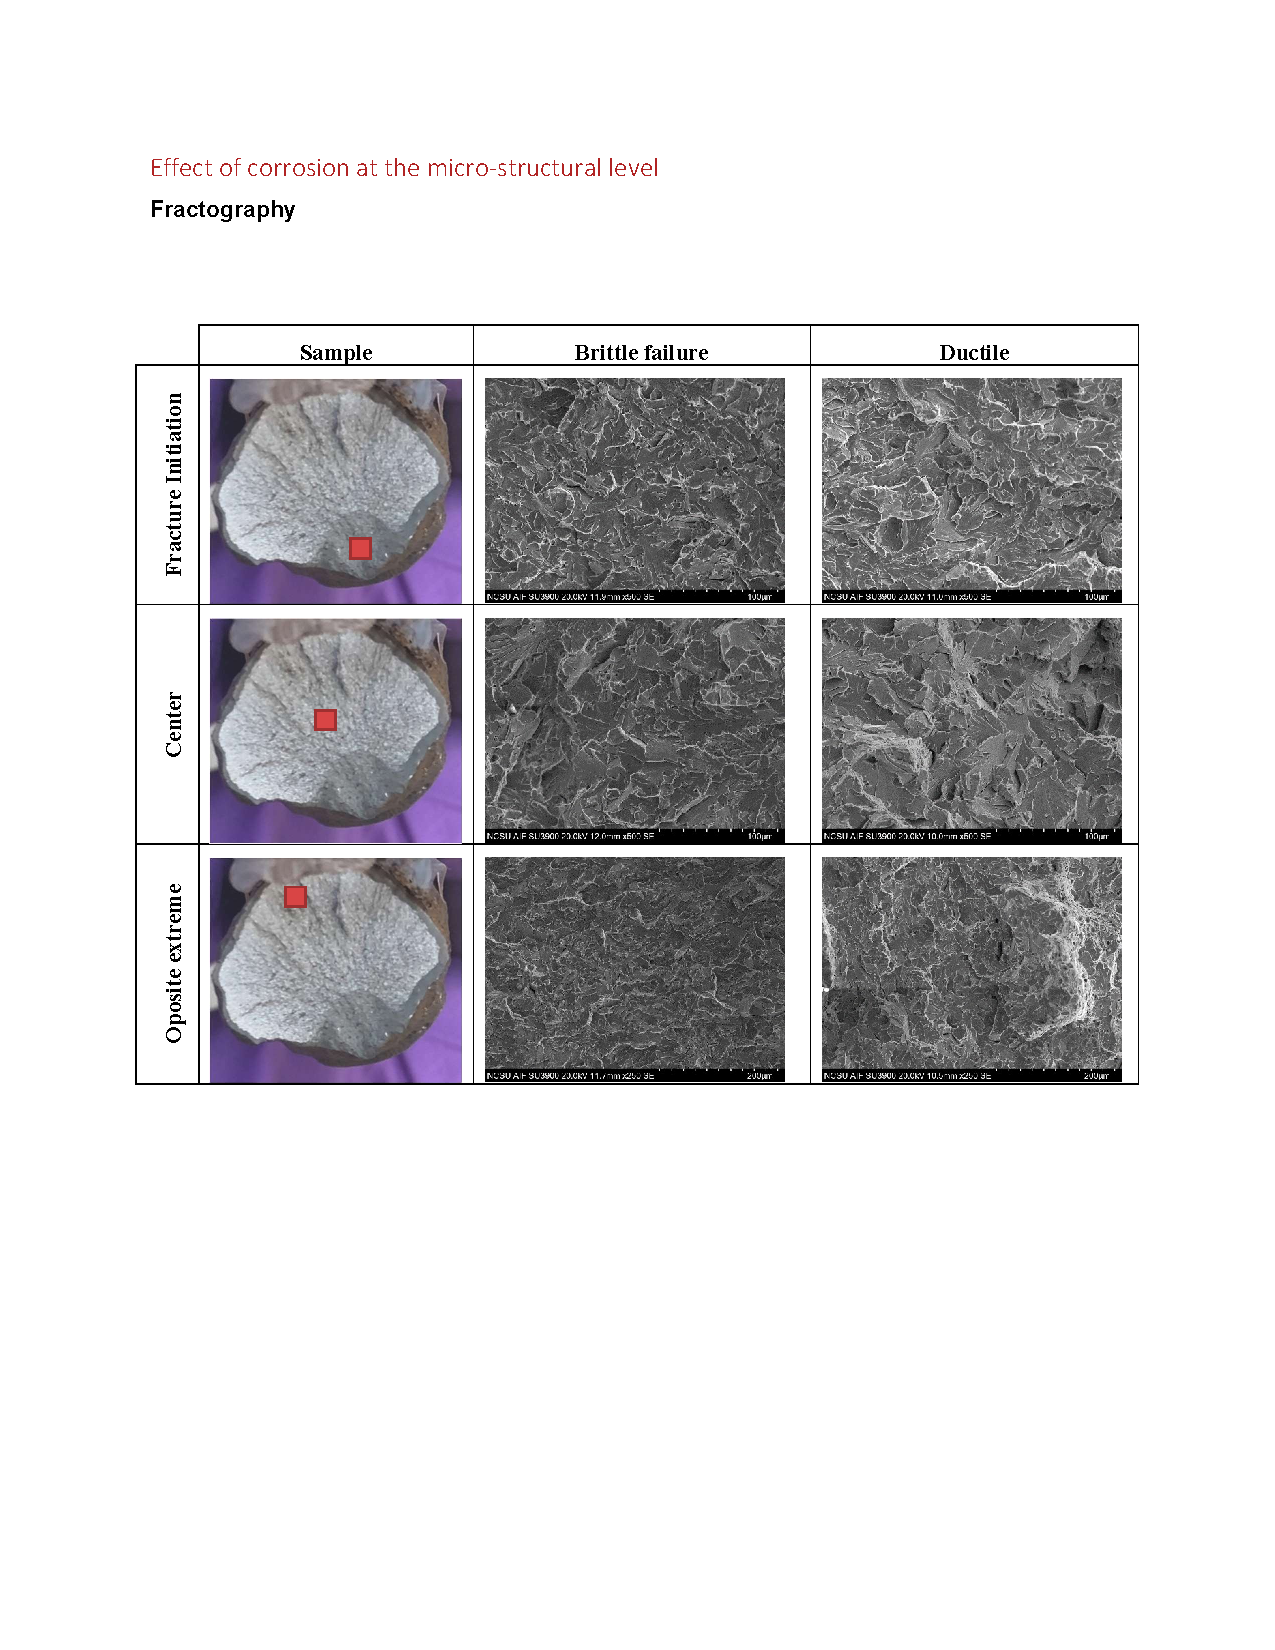
\includegraphics[width=1\textwidth]{VAC Thesis 2.0/Chapter-4/figs/BBT_fractography.pdf}
	\caption{SEM observations for brittle and ductile failure at different positions of the fracture surface}
	\label{fig:FractureSurfaces}
\end{figure}

An important feature from the images obtained in the VPSEM observations was river-like features observed through all the points of observations, as shown in \fref{fig:RiverFeatures}. These types of features are typical of cyclic fatigue tests, which is coherent with the BBT tests since the bar is loaded in compression and then loaded in tension.

\begin{figure}[htbp]
	\centering
	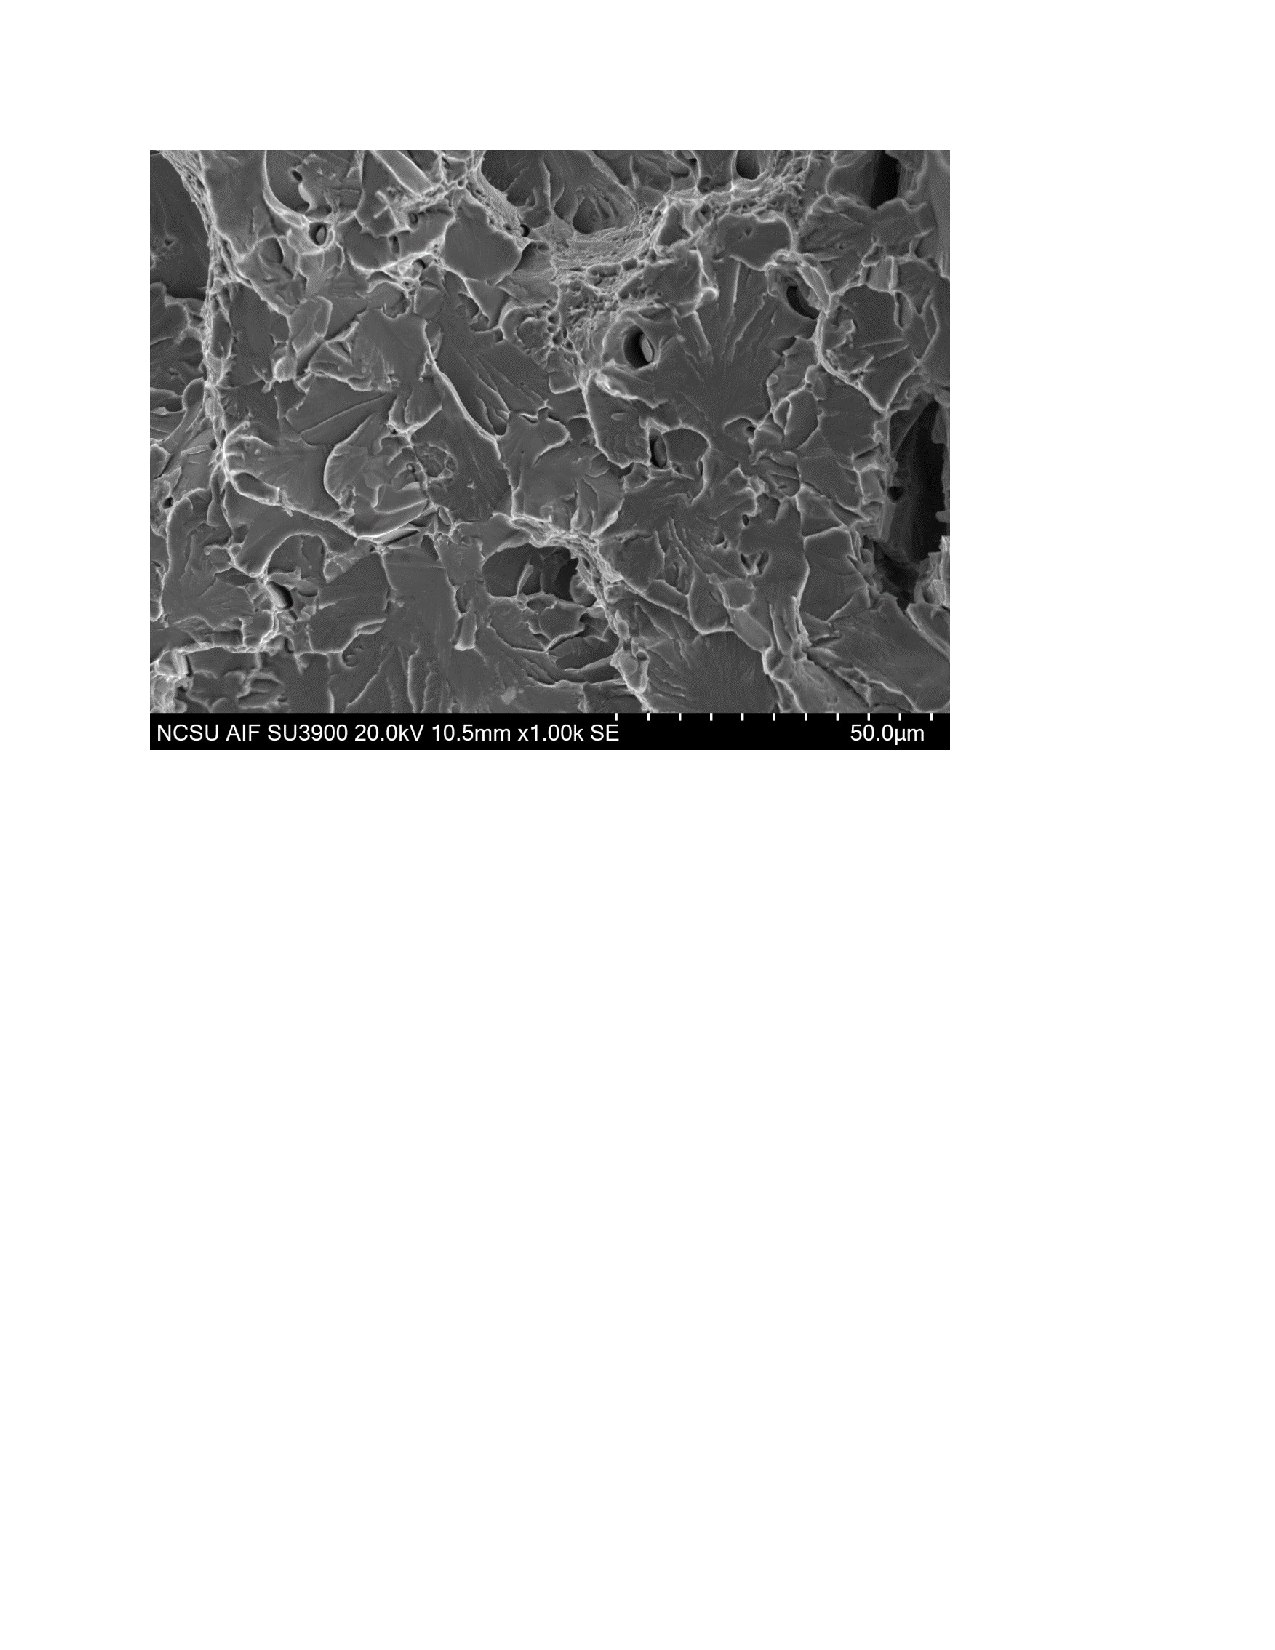
\includegraphics[width=0.7\textwidth]{VAC Thesis 2.0/Chapter-4/figs/BBT_RiverFeatures.pdf}
	\caption{SEM cyclic loading features on fracture surface at 500x magnification}
	\label{fig:RiverFeatures}
\end{figure}

\textbf{Spectrum analysis}

In order to rule out the preclusion to failure due to inclusion of chlorides in the fracture surface, Back Scatter Electron (BSE) SEM images were evaluated through the use of spectrum analysis of the X-ray energy of the fracture surface. \fref{fig:SpectrumAnalysis} shows the spectrum analysis of a brittle and ductile sample. The results obtained show elements that are expected on alloyed steel such as iron (Fe), carbon (C), chromium (Cr), manganese (Mn), and vanadium (V), among others. But no presence of chlorides (such as NaCl) or oxides (such as FeO) was detected. Thus, we are able to rule out the onset of fracture due to the presence of these compounds.

\begin{figure}[htbp]
	\centering
	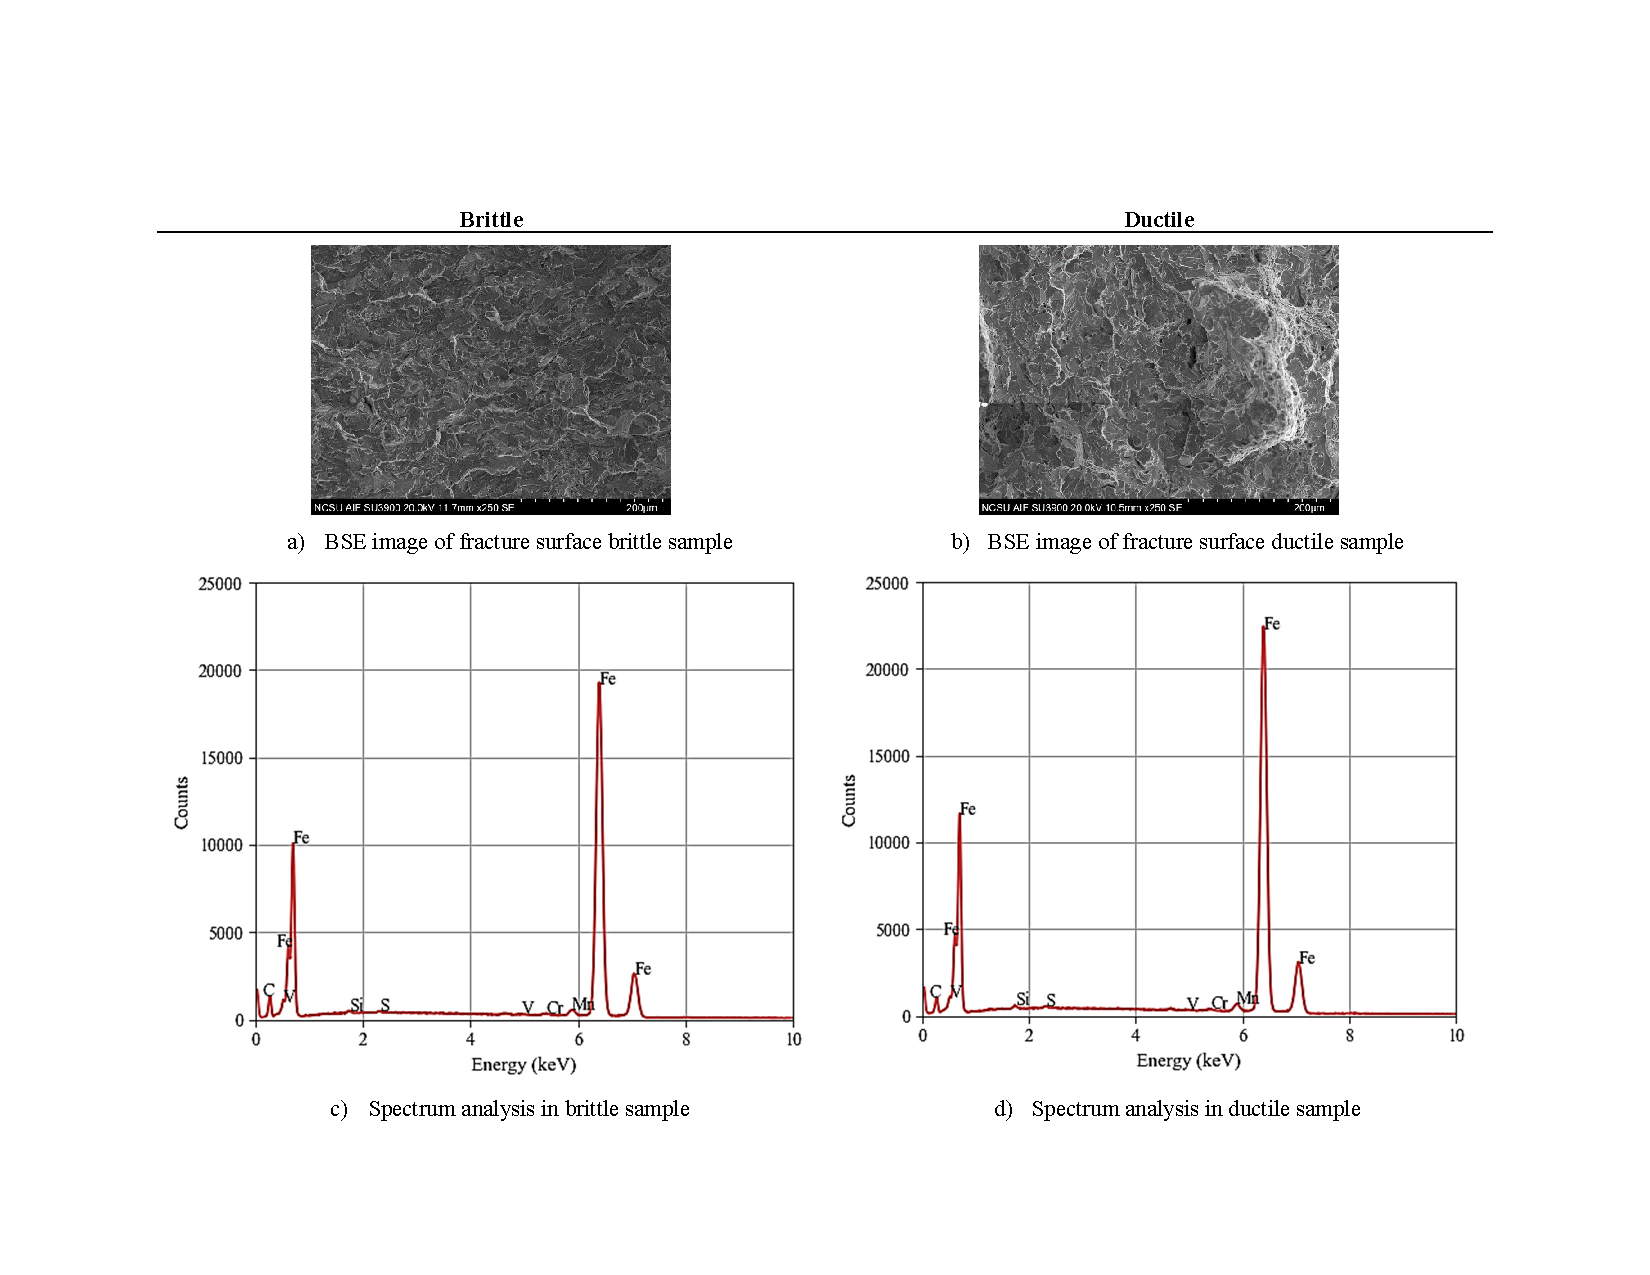
\includegraphics[width=0.84\textwidth]{VAC Thesis 2.0/Chapter-4/figs/BBT_SpectrumAnalysis.pdf}
	\caption{Spectrum analysis of back scatter electrons (BSE) imaging of fracture surface for brittle and ductile failures}
	\label{fig:SpectrumAnalysis}
\end{figure}

\newpage

\section{Tests on Turned Down Corroded Rebars}

\section{Discussion of Results}

The experimental program in this study found the following results:

The use of the effective diameter is a reliable tool to estimate the corrosion level based on geometrical measurements. The use of an effective diameter is especially useful in the case of field measurements taken from corroded rebars. 

The basis for a good assessment is how well the probable properties of the structural materials are. Therefore, the availability of the effective mechanical properties for corroded reinforcing steel provides a great tool to estimate the residual strength and residual ductility to an extent of corroded structures. In addition, the use of the maximum bending strain to obtain the maximum ductility capacity is a good contribution since we can relate the maximum bending strain to the ultimate limit state. This model is replicated here as \eref{eq.BarFracture} developed by Barcley et al \cite{Barcley2019}.This model was implemented in the analytical model presented in Chapter \ref{chap-five}. 

\begin{equation}
    \varepsilon_{t}=\frac{ln(\frac{\varepsilon_{b}}{0.001})}{\frac{300p}{f'c A_{g}}+\frac{0.7}{\rho_{t}}}
    \label{eq.BarFracture}
\end{equation}

The use of SEM observations for specific goals proved very useful since this study determined that the microstructural integrity of the material is not changed or affected by any inclusion of chlorides in the fracture surface, but rather shows a geometrical effect of the imperfections of the corroded surface of the rebar. These imperfections act as stress risers and preclude an earlier failure of the reinforcing steel. These results became more evident as we removed the imperfections. We can observe that both the tension tests and BBT tests show that the virgin metal in the reinforcing steel remains unchanged and unaffected by the corrosion.


%------
% For BBT test results
%The selection for each prescribed bending strains consist of 1) Start with the maximum bending strain determined in previous research to be around $\varepsilon=0.10$ as shown in \fref{fig:BBT_MaxBendingStrain}, 2)if brittle fracture is observed the next test will be at a lower bending strain for example $\varepsilon=0.08$, 3)otherwise higher strains such as $\varepsilon=0.12$ will be evaluated. This is repeated for each corrosion level.

%\section{Expected outcomes from experimental phase}
%
%The results from the tension tests will help to establish if the depassivation process in the corroded rebars has an effect on the measured stress-strain relationship of steel as has been observed in previous research that did not considered the depassivation process \cite{Meda2014},\cite{Yuan2017a},\cite{Du2005}. Similarly the results from the BBT tests will show any changes in the critical bending strain of rebars as they corrode. The critical bending train impacts the bar fracture limit state. In the case of corroded rebars it is expected that the critical bending strain will be modified by changes in the mechanical properties of steel due to corrosion, and effects of concentrated corrosion will be visible along the surface of the rebars. We hypothesize that these two factors will induce fracture at a lower bending strain than those observed in pristine conditions rebars\cite{Barcley2019}.
%
%The results obtained from the experiment will also be used to define the bar fracture limit state for RC columns. Research currently being developed at NC State will provide models that allow us to establish bar fracture tensile strain while considering different parameters such as transverse steel spacing, axial load ratio, and strength of the concrete to mention a few. The model will be similar to that presented by Barcley et al \cite{Barcley2018} shown in \eref{eq.BarFracture}. 
%\begin{equation}
%    \varepsilon_{t}=\frac{ln(\frac{\varepsilon_{b}}{0.001})}{\frac{300p}{f'c A_{g}}+\frac{0.7}{\rho_{t}}}
%    \label{eq.BarFracture}
%\end{equation}
%This model could then be implemented in the analytical model presented in Chapter \ref{chap-four}. If fracture occurs at a lower strain in corroded rebars, this implies that the corroded RC columns are prone to reach the fracture bar limit state at a much lower displacement than in a pristine RC column.
%
%Future studies will verify the application of the results found in this research to perform full scale corroded RC column that consider the effect of depassivation in the cyclic behavior of such columns.